% Options for packages loaded elsewhere
\PassOptionsToPackage{unicode}{hyperref}
\PassOptionsToPackage{hyphens}{url}
\PassOptionsToPackage{dvipsnames,svgnames,x11names}{xcolor}
%
\documentclass[
  letterpaper,
  DIV=11,
  numbers=noendperiod]{scrartcl}

\usepackage{amsmath,amssymb}
\usepackage{iftex}
\ifPDFTeX
  \usepackage[T1]{fontenc}
  \usepackage[utf8]{inputenc}
  \usepackage{textcomp} % provide euro and other symbols
\else % if luatex or xetex
  \usepackage{unicode-math}
  \defaultfontfeatures{Scale=MatchLowercase}
  \defaultfontfeatures[\rmfamily]{Ligatures=TeX,Scale=1}
\fi
\usepackage{lmodern}
\ifPDFTeX\else  
    % xetex/luatex font selection
\fi
% Use upquote if available, for straight quotes in verbatim environments
\IfFileExists{upquote.sty}{\usepackage{upquote}}{}
\IfFileExists{microtype.sty}{% use microtype if available
  \usepackage[]{microtype}
  \UseMicrotypeSet[protrusion]{basicmath} % disable protrusion for tt fonts
}{}
\makeatletter
\@ifundefined{KOMAClassName}{% if non-KOMA class
  \IfFileExists{parskip.sty}{%
    \usepackage{parskip}
  }{% else
    \setlength{\parindent}{0pt}
    \setlength{\parskip}{6pt plus 2pt minus 1pt}}
}{% if KOMA class
  \KOMAoptions{parskip=half}}
\makeatother
\usepackage{xcolor}
\setlength{\emergencystretch}{3em} % prevent overfull lines
\setcounter{secnumdepth}{5}
% Make \paragraph and \subparagraph free-standing
\ifx\paragraph\undefined\else
  \let\oldparagraph\paragraph
  \renewcommand{\paragraph}[1]{\oldparagraph{#1}\mbox{}}
\fi
\ifx\subparagraph\undefined\else
  \let\oldsubparagraph\subparagraph
  \renewcommand{\subparagraph}[1]{\oldsubparagraph{#1}\mbox{}}
\fi

\usepackage{color}
\usepackage{fancyvrb}
\newcommand{\VerbBar}{|}
\newcommand{\VERB}{\Verb[commandchars=\\\{\}]}
\DefineVerbatimEnvironment{Highlighting}{Verbatim}{commandchars=\\\{\}}
% Add ',fontsize=\small' for more characters per line
\usepackage{framed}
\definecolor{shadecolor}{RGB}{241,243,245}
\newenvironment{Shaded}{\begin{snugshade}}{\end{snugshade}}
\newcommand{\AlertTok}[1]{\textcolor[rgb]{0.68,0.00,0.00}{#1}}
\newcommand{\AnnotationTok}[1]{\textcolor[rgb]{0.37,0.37,0.37}{#1}}
\newcommand{\AttributeTok}[1]{\textcolor[rgb]{0.40,0.45,0.13}{#1}}
\newcommand{\BaseNTok}[1]{\textcolor[rgb]{0.68,0.00,0.00}{#1}}
\newcommand{\BuiltInTok}[1]{\textcolor[rgb]{0.00,0.23,0.31}{#1}}
\newcommand{\CharTok}[1]{\textcolor[rgb]{0.13,0.47,0.30}{#1}}
\newcommand{\CommentTok}[1]{\textcolor[rgb]{0.37,0.37,0.37}{#1}}
\newcommand{\CommentVarTok}[1]{\textcolor[rgb]{0.37,0.37,0.37}{\textit{#1}}}
\newcommand{\ConstantTok}[1]{\textcolor[rgb]{0.56,0.35,0.01}{#1}}
\newcommand{\ControlFlowTok}[1]{\textcolor[rgb]{0.00,0.23,0.31}{#1}}
\newcommand{\DataTypeTok}[1]{\textcolor[rgb]{0.68,0.00,0.00}{#1}}
\newcommand{\DecValTok}[1]{\textcolor[rgb]{0.68,0.00,0.00}{#1}}
\newcommand{\DocumentationTok}[1]{\textcolor[rgb]{0.37,0.37,0.37}{\textit{#1}}}
\newcommand{\ErrorTok}[1]{\textcolor[rgb]{0.68,0.00,0.00}{#1}}
\newcommand{\ExtensionTok}[1]{\textcolor[rgb]{0.00,0.23,0.31}{#1}}
\newcommand{\FloatTok}[1]{\textcolor[rgb]{0.68,0.00,0.00}{#1}}
\newcommand{\FunctionTok}[1]{\textcolor[rgb]{0.28,0.35,0.67}{#1}}
\newcommand{\ImportTok}[1]{\textcolor[rgb]{0.00,0.46,0.62}{#1}}
\newcommand{\InformationTok}[1]{\textcolor[rgb]{0.37,0.37,0.37}{#1}}
\newcommand{\KeywordTok}[1]{\textcolor[rgb]{0.00,0.23,0.31}{#1}}
\newcommand{\NormalTok}[1]{\textcolor[rgb]{0.00,0.23,0.31}{#1}}
\newcommand{\OperatorTok}[1]{\textcolor[rgb]{0.37,0.37,0.37}{#1}}
\newcommand{\OtherTok}[1]{\textcolor[rgb]{0.00,0.23,0.31}{#1}}
\newcommand{\PreprocessorTok}[1]{\textcolor[rgb]{0.68,0.00,0.00}{#1}}
\newcommand{\RegionMarkerTok}[1]{\textcolor[rgb]{0.00,0.23,0.31}{#1}}
\newcommand{\SpecialCharTok}[1]{\textcolor[rgb]{0.37,0.37,0.37}{#1}}
\newcommand{\SpecialStringTok}[1]{\textcolor[rgb]{0.13,0.47,0.30}{#1}}
\newcommand{\StringTok}[1]{\textcolor[rgb]{0.13,0.47,0.30}{#1}}
\newcommand{\VariableTok}[1]{\textcolor[rgb]{0.07,0.07,0.07}{#1}}
\newcommand{\VerbatimStringTok}[1]{\textcolor[rgb]{0.13,0.47,0.30}{#1}}
\newcommand{\WarningTok}[1]{\textcolor[rgb]{0.37,0.37,0.37}{\textit{#1}}}

\providecommand{\tightlist}{%
  \setlength{\itemsep}{0pt}\setlength{\parskip}{0pt}}\usepackage{longtable,booktabs,array}
\usepackage{calc} % for calculating minipage widths
% Correct order of tables after \paragraph or \subparagraph
\usepackage{etoolbox}
\makeatletter
\patchcmd\longtable{\par}{\if@noskipsec\mbox{}\fi\par}{}{}
\makeatother
% Allow footnotes in longtable head/foot
\IfFileExists{footnotehyper.sty}{\usepackage{footnotehyper}}{\usepackage{footnote}}
\makesavenoteenv{longtable}
\usepackage{graphicx}
\makeatletter
\def\maxwidth{\ifdim\Gin@nat@width>\linewidth\linewidth\else\Gin@nat@width\fi}
\def\maxheight{\ifdim\Gin@nat@height>\textheight\textheight\else\Gin@nat@height\fi}
\makeatother
% Scale images if necessary, so that they will not overflow the page
% margins by default, and it is still possible to overwrite the defaults
% using explicit options in \includegraphics[width, height, ...]{}
\setkeys{Gin}{width=\maxwidth,height=\maxheight,keepaspectratio}
% Set default figure placement to htbp
\makeatletter
\def\fps@figure{htbp}
\makeatother

\usepackage{booktabs}
\usepackage{longtable}
\usepackage{array}
\usepackage{multirow}
\usepackage{wrapfig}
\usepackage{float}
\usepackage{colortbl}
\usepackage{pdflscape}
\usepackage{tabu}
\usepackage{threeparttable}
\usepackage{threeparttablex}
\usepackage[normalem]{ulem}
\usepackage{makecell}
\usepackage{xcolor}
\usepackage{lipsum}
\usepackage{setspace}
\onehalfspacing
\linespread{2}
\KOMAoption{captions}{tableheading}
\makeatletter
\@ifpackageloaded{caption}{}{\usepackage{caption}}
\AtBeginDocument{%
\ifdefined\contentsname
  \renewcommand*\contentsname{Table of contents}
\else
  \newcommand\contentsname{Table of contents}
\fi
\ifdefined\listfigurename
  \renewcommand*\listfigurename{List of Figures}
\else
  \newcommand\listfigurename{List of Figures}
\fi
\ifdefined\listtablename
  \renewcommand*\listtablename{List of Tables}
\else
  \newcommand\listtablename{List of Tables}
\fi
\ifdefined\figurename
  \renewcommand*\figurename{Figure}
\else
  \newcommand\figurename{Figure}
\fi
\ifdefined\tablename
  \renewcommand*\tablename{Table}
\else
  \newcommand\tablename{Table}
\fi
}
\@ifpackageloaded{float}{}{\usepackage{float}}
\floatstyle{ruled}
\@ifundefined{c@chapter}{\newfloat{codelisting}{h}{lop}}{\newfloat{codelisting}{h}{lop}[chapter]}
\floatname{codelisting}{Listing}
\newcommand*\listoflistings{\listof{codelisting}{List of Listings}}
\makeatother
\makeatletter
\makeatother
\makeatletter
\@ifpackageloaded{caption}{}{\usepackage{caption}}
\@ifpackageloaded{subcaption}{}{\usepackage{subcaption}}
\makeatother
\ifLuaTeX
  \usepackage{selnolig}  % disable illegal ligatures
\fi
\usepackage{bookmark}

\IfFileExists{xurl.sty}{\usepackage{xurl}}{} % add URL line breaks if available
\urlstyle{same} % disable monospaced font for URLs
\hypersetup{
  pdftitle={ATP and WTA Professional Tennis: Calculating In-Match-Win Probability with Bayesian Modeling},
  pdfauthor={Ben Moolman},
  colorlinks=true,
  linkcolor={blue},
  filecolor={Maroon},
  citecolor={Blue},
  urlcolor={Blue},
  pdfcreator={LaTeX via pandoc}}

\title{ATP and WTA Professional Tennis: Calculating In-Match-Win
Probability with Bayesian Modeling}
\author{Ben Moolman}
\date{}

\begin{document}
\maketitle

\renewcommand*\contentsname{Table of contents}
{
\hypersetup{linkcolor=}
\setcounter{tocdepth}{3}
\tableofcontents
}
\linespread{0.9}

\linespread{2}

\subsection{Introduction}\label{introduction}

In this project, we explore the in-match-win probability of professional
tennis matches. Tennis' scoring format allows for huge momentum swings
in a short amount of time. We are going to explore how the probabilities
that tennis players win a match are calculated and update throughout the
match using Bayesian modeling. To determine the probability that a
player (player 1) wins a match against another player (player 2), we
incorporate (1) the probability that player 1 wins a point on serve
against player 2, (2) the probability that player 2 wins a point on
serve against player 1, and (3) the current score of the match of
interest. The prior distributions for (1) and (2) are generated from
points played in matches prior to the match of interest. Both (1) and
(2) are then updated throughout the match of interest as points played
between the two players update their prior point-win probabilities. As
case studies, we explore the 2022 Men's US Open Quarterfinal between
Carlos Alcaraz and Jannik Sinner and the 2023 Women's US Open Final
between Coco Gauff and Arnya Sabalenka.

\subsubsection{Outline}\label{outline}

We begin by exploring tennis scoring to get an understanding of how a
match is played in Section~\ref{sec-scoring}. We then look at the data
we are using in this project on Section~\ref{sec-data}. Then, in
Section~\ref{sec-bayesianmod}, we discuss Bayesian modeling, and come up
with our probabilities of the players winning a point on their serves
against specific opponents. We calculate the in-match-win probability
and how we update our prior distributions throughout the match. We then
look at the case studies of the 2022 Men's US Open Quarterfinal between
Carlos Alcaraz and Jannik Sinner, and discuss how we can change what
matches we include in our prior distribution in Section~\ref{sec-alcsin}
and Section~\ref{sec-changeprior}. We also explore the 2023 Women's US
Open Final between Coco Gauff and Aryna Sabalenka in
Section~\ref{sec-gauffsab}. We conclude in Section~\ref{sec-conclusion}
with a discussion of the results and potential future work. An appendix
in Section~\ref{sec-appendix} is included with the code used in this
project for reference.

\subsubsection{Tennis Scoring}\label{sec-scoring}

The scoring format in tennis can be confusing to those that are not
familiar with the sport. Below is a brief outline of how tennis matches
are scored:

\begin{itemize}
\tightlist
\item
  The match starts with one player serving at 0-0
\item
  The server is the player that hits the ball first in a point
\item
  The server alternates what direction they serve from after every point
  (deuce side and ad side)
\item
  A game is played with the server serving for the entire game
\item
  A game is won by the first player to win 4 points, wining by a margin
  of 2 or more points
\item
  Sets are played first to 6 games, wining by a margin of 2 or more
  games
\item
  If the score reaches 6-6 in a set, a tiebreak is played
\item
  A tiebreak is won by the first player to win 7 points, wining by a
  margin of 2 or more points
\item
  A match is played to the best of 3 or 5 sets based on the tournament
  format
\end{itemize}

A little more tennis terminology are the words break and hold, defined
below:

\begin{itemize}
\tightlist
\item
  Break: when the player returning wins the game
\item
  Hold: when the player serving wins the game
\end{itemize}

A graphic is attached below to help, and a more detailed write-up can be
found on the website \emph{doubletake}
\href{https://www.shopdoubletake.com/blogs/well-played/tennis-scoring-101}{here}.

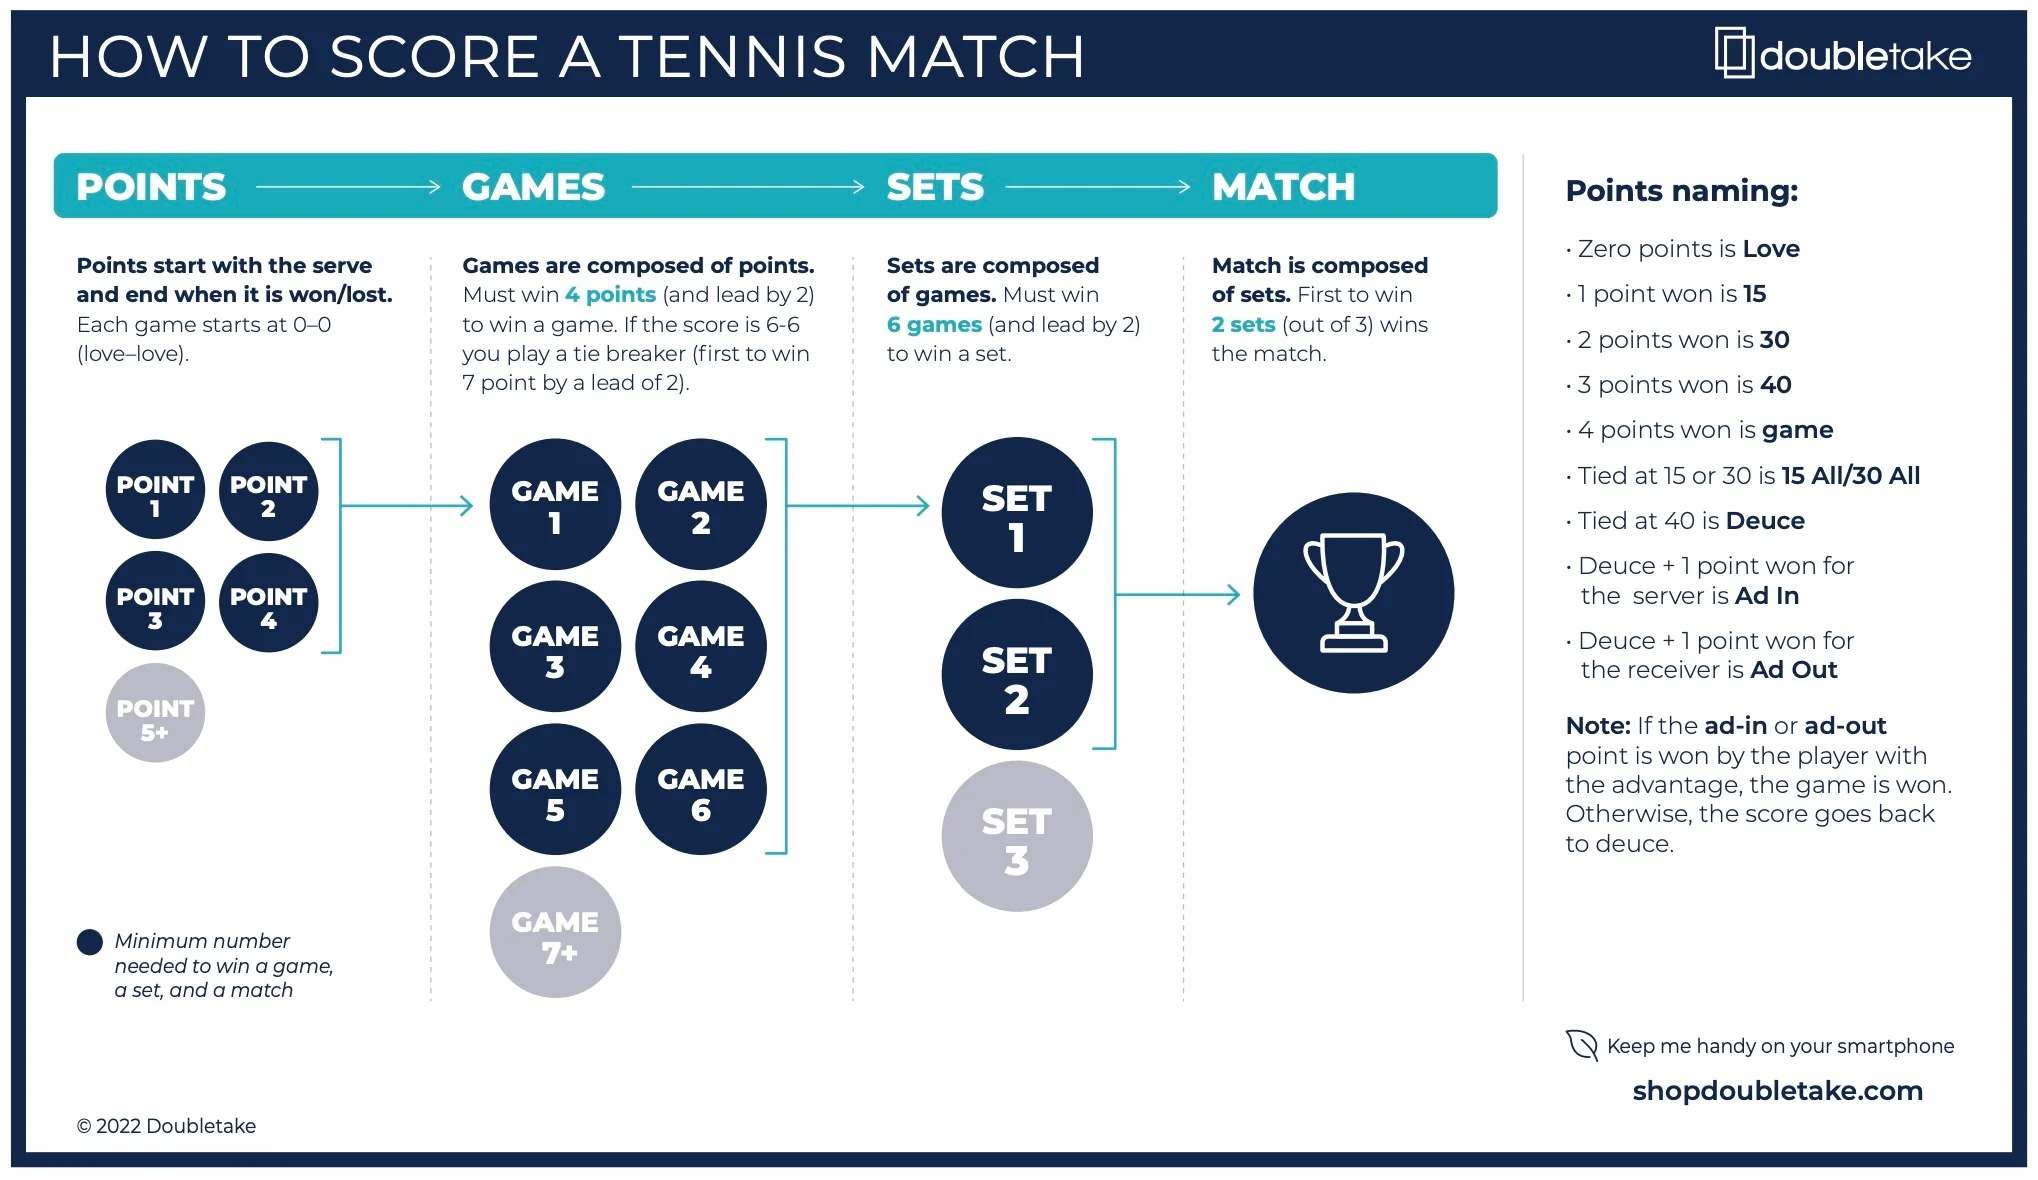
\includegraphics{tennis_scoring.jpeg}

\subsubsection{Data}\label{sec-data}

The data used in this project is from the ATP and WTA professional
tennis tours, and is from Jeff Sackman's tennis data on Github. There is
\href{https://github.com/JeffSackmann/tennis_slam_pointbypoint}{point-level
data} on the ATP and WTA main-draw singles grand slam tournaments from
2011-present. There is also
\href{https://github.com/JeffSackmann/tennis_atp}{match-level data} for
ATP matches and
\href{https://github.com/JeffSackmann/tennis_wta}{match-level data} for
WTA matches. Access to the data is needed to ensure correct spelling of
player names (especially nicknames, ie ``Rafa Nadal'' vs ``Rafael
Nadal'') and tournament names, the correct date ranges, file paths, and
match IDs for specific matches of interest. Checking these details is
best done on the matches data frames, and if finding the information on
the Github site is problematic, the data can be read in using the
\texttt{read\_matches()} function, which works for both ATP and WTA
data.

We can explore what the data containing all of the matches looks like.
Here we look at one match from the first round of the 2022 Men's US
Open. This is one row of the data frame but is shown over multiple rows
here for readability.

\linespread{0.9}

\linespread{2}

We can explore some of the point level data to get a better
understanding of what we are working with. Below are some selected rows
from the point-level data once we have cleaned it and tidied it for what
we need. This data is taken from the 2022 Men's US Open Quarterfinal
between Carlos Alcaraz and Jannik Sinner.

\linespread{0.9}

\linespread{2}

The first 10 points from the start of the match, where we see Alcaraz
break Sinner's serve in the first game of the match, are shown in the
table below:

\linespread{0.9}

\begingroup\fontsize{11}{13}\selectfont

\begin{longtable*}[t]{rrrllrrrr}
\toprule
pt\_number & PointServer & PointWinner & P1Score & P2Score & P1GamesWon & P2GamesWon & P1SetsWon & P2Setswon\\
\midrule
1 & 1 & 2 & 0 & 15 & 0 & 0 & 0 & 0\\
2 & 1 & 1 & 15 & 15 & 0 & 0 & 0 & 0\\
3 & 1 & 2 & 15 & 30 & 0 & 0 & 0 & 0\\
4 & 1 & 1 & 30 & 30 & 0 & 0 & 0 & 0\\
5 & 1 & 2 & 30 & 40 & 0 & 0 & 0 & 0\\
\addlinespace
6 & 1 & 1 & 40 & 40 & 0 & 0 & 0 & 0\\
7 & 1 & 2 & 40 & AD & 0 & 0 & 0 & 0\\
8 & 1 & 1 & 40 & 40 & 0 & 0 & 0 & 0\\
9 & 1 & 2 & 40 & AD & 0 & 0 & 0 & 0\\
10 & 1 & 2 & 0 & 0 & 0 & 1 & 0 & 0\\
\bottomrule
\end{longtable*}
\endgroup{}

\linespread{2}

We next show some points at the end of the second set, as Sinner wins
the second set tiebreak 9-7:

\linespread{0.9}

\begingroup\fontsize{11}{13}\selectfont

\begin{longtabu} to \linewidth {>{\raggedleft}X>{\raggedleft}X>{\raggedleft}X>{\raggedright}X>{\raggedright}X>{\raggedleft}X>{\raggedleft}X>{\raggedleft}X>{\raggedleft}X}
\toprule
pt\_number & PointServer & PointWinner & P1Score & P2Score & P1GamesWon & P2GamesWon & P1SetsWon & P2Setswon\\
\midrule
143 & 1 & 1 & 0 & 0 & 6 & 6 & 0 & 1\\
144 & 2 & 2 & 0 & 1 & 6 & 6 & 0 & 1\\
145 & 1 & 1 & 1 & 1 & 6 & 6 & 0 & 1\\
146 & 1 & 1 & 2 & 1 & 6 & 6 & 0 & 1\\
147 & 2 & 2 & 2 & 2 & 6 & 6 & 0 & 1\\
\addlinespace
148 & 2 & 2 & 2 & 3 & 6 & 6 & 0 & 1\\
149 & 1 & 1 & 3 & 3 & 6 & 6 & 0 & 1\\
150 & 1 & 1 & 4 & 3 & 6 & 6 & 0 & 1\\
151 & 2 & 1 & 5 & 3 & 6 & 6 & 0 & 1\\
152 & 2 & 2 & 5 & 4 & 6 & 6 & 0 & 1\\
\addlinespace
153 & 1 & 2 & 5 & 5 & 6 & 6 & 0 & 1\\
154 & 1 & 1 & 6 & 5 & 6 & 6 & 0 & 1\\
155 & 2 & 2 & 6 & 6 & 6 & 6 & 0 & 1\\
156 & 2 & 2 & 6 & 7 & 6 & 6 & 0 & 1\\
157 & 1 & 1 & 7 & 7 & 6 & 6 & 0 & 1\\
\addlinespace
158 & 1 & 1 & 8 & 7 & 6 & 6 & 0 & 1\\
159 & 2 & 1 & 0 & 0 & 0 & 0 & 1 & 1\\
160 & 1 & 1 & 15 & 0 & 0 & 0 & 1 & 1\\
161 & 1 & 1 & 30 & 0 & 0 & 0 & 1 & 1\\
162 & 1 & 1 & 40 & 0 & 0 & 0 & 1 & 1\\
\bottomrule
\end{longtabu}
\endgroup{}

\linespread{2}

\subsection{Bayesian Modeling}\label{sec-bayesianmod}

We next give a brief overview of Bayesian modeling before discussing how
the framework is applied to our project on in-match-win probability.

\subsubsection{Brief Overview}\label{brief-overview}

In Bayesian modeling, we start with some existing beliefs about a
parameter, which we call our prior distribution for that parameter. We
then observe new data come in and update our beliefs about the parameter
based on the new data, which we call our posterior distribution.

In this project, our parameters of interest are the probabilities that
player1 and player2 win a point on their serve. We calculate these
probabilities using previous matches that have been played. As the match
progresses, we update our beliefs about these probabilities of winning a
point on serve, and at a specific state of the match, we can calculate
the probability that either of the players wins the match. Choosing
which matches we include in our prior distributions is important, as we
want to include matches that are relevant to the match of interest.

Throughout this paper, we use the 2022 Men's US Open Quarterfinal match
between Carlos Alcaraz and Jannik Sinner as an example match to make
discussing the Bayesian model more straightforward. So, in the context
of this match, our parameters of interest are the probabilities that
Alcaraz wins a point on his serve against Sinner, and the probability
that Sinner wins a point on his serve against Alcaraz. After each point
of their quarterfinal match is played, we update these probability
distributions.

\subsubsection{Matches for Prior
Distributions}\label{matches-for-prior-distributions}

We start with some prior beliefs about the probabilities that Alcaraz
and Sinner win a point on serve. We use the data from previous matches
to calculate these prior distributions. These matches we choose to
include in our prior distributions are important, as we want to include
matches that are relevant to the match of interest. The matches that we
choose to include for this example include both matches that Alcaraz and
Sinner have played in, as well as matches that other players have played
in.

\linespread{0.9}

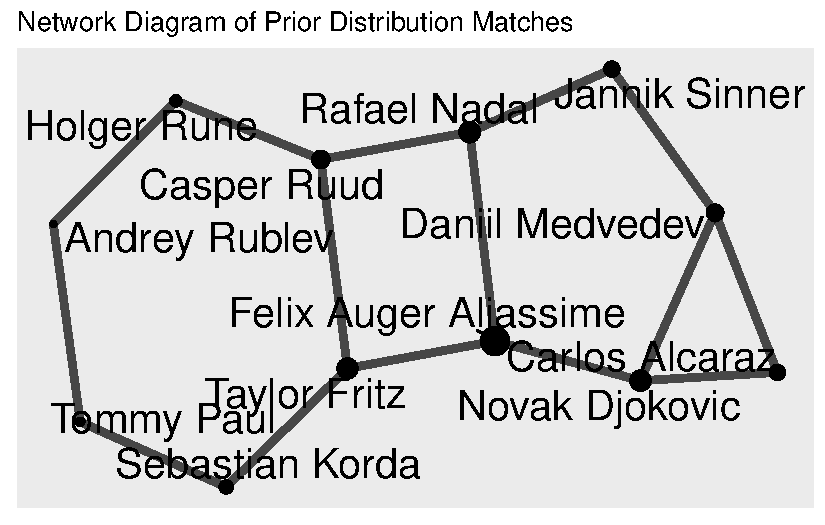
\includegraphics{Project_Write_Up_files/figure-pdf/unnamed-chunk-7-1.pdf}

\linespread{2}

This network diagram is an example of a group of matches that can be
used to form a prior distribution. Note that these are not the actual
matches we include to form the prior distribution but are instead just
made-up match-ups to illustrate a possible network of matches.

In the diagram, the nodes represent players, and the edges represent
matches that have been played. We can see that Jannik Sinner and Carlos
Alcaraz have not played a match against each other out of the
(hypothetical) matches included here. However, we are still able to
calculate their probabilities of winning a point on serve against each
other by using the data from the matches that they have played in, as
well as the matches that other players have played in, because there is
a ``path'' between Sinner and Alcaraz (the most direct path in this
example goes through Medvedev).

For example, we would not be able to use just the early rounds of the
2022 US Open to form a prior distribution for the quarterfinal matchup
between Alcaraz and Sinner. This is because there is no connection
between the two players in the early rounds of the tournament, as nobody
in Alcaraz's section of the draw has played anyone in Sinner's section
of the draw. We would need to include matches that have a connection
between Alcaraz and Sinner, even if they have not played against each
other directly.

\subsubsection{Paired Competition Model}\label{paired-competition-model}

When forming our prior beliefs, we are using a paired competition model.
This means that we are using data from the matches that Alcaraz and
Sinner have played in, as well as other players that they have played
against. For this to work, we need there to be some connection between
Alcaraz and Sinner using matches they and other opponents have played
(ie Sinner has played against player A, who played against player B, who
played against Alcaraz).

We define \(Y_{ijk}\) to be a Bernoulli random variable equal to either:
* \(1\) if player \(i\) wins the \(k^{th}\) point against player \(j\) *
\(0\) if player \(i\) loses the \(k^{th}\) point against player \(j\)

Then \(\text{E}(Y_{ijk}) \equiv \pi_{ijk}\), the probability that Player
\(i\) wins the \(k^{th}\) point against Player \(j\).

So for calculating this in regards to Alcaraz and Sinner and all matches
we include in the prior we have:
\[\text{logit}(\pi_{ijk}) = \beta_{alcaraz}X_{alcaraz} + \beta_{sinner}X_{sinner} + \ldots + \beta_{ruud}X_{ruud}\]

where, for example, \(X_{alcaraz}\) is equal to:

\begin{itemize}
\tightlist
\item
  \(1\) if Alcaraz is player \(i\) on the \(k^{th}\) point
\item
  \(0\) if Alcaraz is neither player \(i\) nor player \(j\) on the
  \(k^{th}\) point
\item
  \(-1\) if Alcaraz is player \(j\) on the \(k^{th}\) point
\end{itemize}

and \(\beta_{alcaraz}\) represents a unitless ``ability'' of Alcaraz.

For an example, the log-odds of Carlos Alcaraz (player \(i\)) winning a
point against Jannik Sinner (player \(j\)):

\begin{equation}
  \begin{aligned}
    \text{logit}(\pi_{ij}) & = \beta_{alcaraz}(1) + \beta_{sinner}(-1) + \ldots + \beta_{ruud}(0) \\
                                 & = \beta_{alcaraz} - \beta_{sinner}
  \end{aligned}
\end{equation}

We can then work on adding a serving effect:

\begin{equation}
  \begin{aligned}
    \text{logit}(\pi_{ijk}) = & \beta_{alcaraz}X_{alcaraz} + \beta_{sinner}X_{sinner} + \ldots + \beta_{ruud}X_{ruud} + \\
    & \alpha_{alcaraz}X_{alcaraz,s} + \alpha_{sinner}X_{sinner,s} + \ldots + \alpha_{ruud}X_{ruud,s}
  \end{aligned},
\end{equation}

where, for example, \(X_{alcaraz,s}\) is equal to:

\begin{itemize}
\tightlist
\item
  \(1\) if Alcaraz is the serving player \(i\) on point \(k\).
\item
  \(0\) if Alcaraz is the returning player on point \(k\) or if Alcaraz
  is neither player \(i\) nor player \(j\).
\item
  \(-1\) if Alcaraz is the serving player \(j\) on point \(k\)
\end{itemize}

So, we have \(\alpha_{alcaraz}\) representing a bump in point win
probability for when Alcaraz serves compared to when he receives.

As an example, the log-odds of Carlos Alcaraz (player \(i\)) winning a
point against Jannik Sinner (player \(j\)) with Alcaraz serving on point
\(k\) would be:

\begin{equation}
  \begin{aligned}
    \text{logit}(\pi_{ijk}) & = \beta_{alcaraz}(1) +       \beta_{sinner}(-1) + \ldots + \beta_{ruud}(0) + \\
    & \;\;\;\; \alpha_{alcaraz}(1) + \alpha_{sinner}(0) + \ldots + \alpha_{ruud}(0) \\
    & = \beta_{alcaraz} + \alpha_{alcaraz} - \beta_{sinner}
  \end{aligned}
\end{equation}

And as another example, the log-odds of Carlos Alcaraz (player \(i\))
winning a point against Jannik Sinner (player \(j\)) with Sinner serving
on point \(k\) would be:

\begin{equation}
  \begin{aligned}
    \text{logit}(\pi_{ijk}) & = \beta_{alcaraz}(1) +       \beta_{sinner}(-1) + \ldots + \beta_{ruud}(0) + \\
    & \;\;\;\; \alpha_{alcaraz}(0) + \alpha_{sinner}(-1) + \ldots + \alpha_{ruud}(0) \\
    & = \beta_{alcaraz} - \beta_{sinner} - \alpha_{sinner}
  \end{aligned}
\end{equation}

We use the data from the lead-up tournaments to the 2022 US Open (hard
court tournaments) and the rounds of the 2022 US Open before the
quarterfinals to calculate these coefficients in the paired competition
model. We can then calculate the log-odds that Alcaraz wins a point
while serving against Sinner, and the log-odds that Sinner wins a point
while serving against Alcaraz. With these estimated log-odds and
standard errors (on the log-odds scale), we then create distributions
for the prior probabilities of winning a point on serve for Alcaraz and
Sinner, assuming that the log-odds of each player winning a point on
serve are normally distributed.

\subsubsection{Calculating the Prior Distributions of Point-win
Probabilities}\label{calculating-the-prior-distributions-of-point-win-probabilities}

Before delving into the details of how to calculate the prior
distributions for the 2022 U.S. Open Quarterfinal match between Alcaraz
and Sinner, we first load in some relevant functions and packages:

\linespread{0.9}

\begin{Shaded}
\begin{Highlighting}[]
\FunctionTok{library}\NormalTok{(tidyverse)}
\FunctionTok{library}\NormalTok{(broom)}
\FunctionTok{library}\NormalTok{(knitr)}
\FunctionTok{library}\NormalTok{(kableExtra)}
\CommentTok{\# install James Wolpe\textquotesingle{}s compr package, run below in console}
\CommentTok{\# devtools::install\_github(repo = "https://github.com/jameswolpe/compr")}
\FunctionTok{library}\NormalTok{(compr)}
\CommentTok{\# install skoval\textquotesingle{}s deuce package, run below in console}
\CommentTok{\# devtools::install\_github("skoval/deuce")}
\FunctionTok{library}\NormalTok{(deuce)}

\FunctionTok{source}\NormalTok{(}\StringTok{"comp\_prior\_start.R"}\NormalTok{)}
\FunctionTok{source}\NormalTok{(}\StringTok{"bayes\_intro.R"}\NormalTok{)}
\FunctionTok{source}\NormalTok{(}\StringTok{"wrangle\_point\_level\_data.R"}\NormalTok{)}
\FunctionTok{source}\NormalTok{(}\StringTok{"create\_prior.R"}\NormalTok{)}
\FunctionTok{source}\NormalTok{(}\StringTok{"get\_probabilities\_df.R"}\NormalTok{)}
\FunctionTok{source}\NormalTok{(}\StringTok{"get\_plot\_df.R"}\NormalTok{)}
\end{Highlighting}
\end{Shaded}

\linespread{2}

To calculate the prior distributions of the probabilities that Alcaraz
and Sinner win a point on serve, we use our \texttt{create\_prior()}
function. Note that this function's outputs are on the log-odds scale,
and contains the mean log-odds values and standard errors, and are also
all in reference to \texttt{player1}, who, in this case, is Jannik
Sinner.

\linespread{0.9}

\begin{Shaded}
\begin{Highlighting}[]
\NormalTok{aug\_mod\_sin\_small\_prior }\OtherTok{\textless{}{-}} \FunctionTok{create\_prior}\NormalTok{(}\AttributeTok{ext =} \FunctionTok{c}\NormalTok{(}\StringTok{"atp\_matches\_2022.csv"}\NormalTok{),}
                         \AttributeTok{tourn\_name =} \StringTok{"Us Open"}\NormalTok{,}
                         \AttributeTok{surf =} \StringTok{"Hard"}\NormalTok{,}
                         \AttributeTok{start\_date =} \StringTok{"2022{-}07{-}25"}\NormalTok{,}
                         \AttributeTok{end\_date =} \StringTok{"2022{-}09{-}06"}\NormalTok{,}
                         \AttributeTok{player1 =} \StringTok{"Jannik Sinner"}\NormalTok{,}
                         \AttributeTok{player2 =} \StringTok{"Carlos Alcaraz"}\NormalTok{,}
                         \AttributeTok{ref\_player =} \StringTok{"Daniil Medvedev"}\NormalTok{)}
\NormalTok{aug\_mod\_sin\_small\_prior }\SpecialCharTok{|\textgreater{}} \FunctionTok{kable}\NormalTok{()}
\end{Highlighting}
\end{Shaded}

\begin{longtable}[]{@{}
  >{\raggedright\arraybackslash}p{(\columnwidth - 10\tabcolsep) * \real{0.2000}}
  >{\raggedright\arraybackslash}p{(\columnwidth - 10\tabcolsep) * \real{0.2143}}
  >{\raggedleft\arraybackslash}p{(\columnwidth - 10\tabcolsep) * \real{0.1429}}
  >{\raggedleft\arraybackslash}p{(\columnwidth - 10\tabcolsep) * \real{0.1429}}
  >{\raggedleft\arraybackslash}p{(\columnwidth - 10\tabcolsep) * \real{0.1571}}
  >{\raggedleft\arraybackslash}p{(\columnwidth - 10\tabcolsep) * \real{0.1429}}@{}}
\toprule\noalign{}
\begin{minipage}[b]{\linewidth}\raggedright
player1
\end{minipage} & \begin{minipage}[b]{\linewidth}\raggedright
player2
\end{minipage} & \begin{minipage}[b]{\linewidth}\raggedleft
p1\_server
\end{minipage} & \begin{minipage}[b]{\linewidth}\raggedleft
p2\_server
\end{minipage} & \begin{minipage}[b]{\linewidth}\raggedleft
.fitted
\end{minipage} & \begin{minipage}[b]{\linewidth}\raggedleft
.se.fit
\end{minipage} \\
\midrule\noalign{}
\endhead
\bottomrule\noalign{}
\endlastfoot
Jannik Sinner & Carlos Alcaraz & 1 & 0 & 0.2434863 & 0.1193404 \\
Jannik Sinner & Carlos Alcaraz & 0 & 1 & -0.5017383 & 0.1196950 \\
\end{longtable}

\linespread{2}

From the output, we see that Sinner has a mean value of winning a point
while serving against Alcaraz of \texttt{0.2434863} with a standard
error of \texttt{0.1193404}, and both of these are on the log-odds
scale. This is indicated by \texttt{p1\_server} being equal to
\texttt{1} for this row. We can also see that Sinner has a mean value of
winning a point while returning against Alcaraz of \texttt{-0.5017383}
with a standard error of \texttt{0.1196950}; again, both are on the
log-odds scale. To get the log-odds of Alcaraz winning a point while
serving against Sinner, we can negate the value of Sinner winning a
point while returning against Alcaraz. We can then convert these from
the log-odds scale to probabilities of winning a point on serve by
backtransforming with \(e^x / (1 + e^x)\), where \(x\) is the log-odds
of winning a point on serve. The function transforms the log-odds to
probabilities, ensuring that the probabilities fall within the range
{[}0, 1{]}.

\linespread{0.9}

\begin{Shaded}
\begin{Highlighting}[]
\DocumentationTok{\#\# probability Sinner wins a point on serve}
\FunctionTok{expit}\NormalTok{(}\FloatTok{0.2434863}\NormalTok{) }\CommentTok{\# 0.5605726}
\end{Highlighting}
\end{Shaded}

\begin{verbatim}
[1] 0.5605726
\end{verbatim}

\begin{Shaded}
\begin{Highlighting}[]
\DocumentationTok{\#\# probability Sinner wins a point on return}
\FunctionTok{expit}\NormalTok{(}\SpecialCharTok{{-}}\FloatTok{0.5017383}\NormalTok{) }\CommentTok{\#  0.3771322}
\end{Highlighting}
\end{Shaded}

\begin{verbatim}
[1] 0.3771322
\end{verbatim}

\begin{Shaded}
\begin{Highlighting}[]
\DocumentationTok{\#\# probability Alcaraz wins a point on serve}
\FunctionTok{expit}\NormalTok{(}\FloatTok{0.5017383}\NormalTok{) }\CommentTok{\# 0.6228678}
\end{Highlighting}
\end{Shaded}

\begin{verbatim}
[1] 0.6228678
\end{verbatim}

\begin{Shaded}
\begin{Highlighting}[]
\DocumentationTok{\#\# probability Alcaraz wins a point on return}
\FunctionTok{expit}\NormalTok{(}\SpecialCharTok{{-}}\FloatTok{0.2434863}\NormalTok{) }\CommentTok{\# 0.4394274}
\end{Highlighting}
\end{Shaded}

\begin{verbatim}
[1] 0.4394274
\end{verbatim}

\linespread{2}

From this prior model, we estimate Sinner to win around 56.06\% of
points played on his serve against Alcaraz, and for Alcaraz to win
around 62.29\% of points played on his serve against Sinner.

We can then create distributions to visualize what these probabilities
look like, assuming normality on the log-odds scale. We will start with
our log-odds and randomly generate 200,000 random samples from a normal
distribution with mean log-odds from our prior and standard errors from
our prior.

\linespread{0.9}

\begin{Shaded}
\begin{Highlighting}[]
\DocumentationTok{\#\# Save sinner log{-}odds and se from prior as variables}
\NormalTok{prior\_sin\_logodds }\OtherTok{\textless{}{-}} \FloatTok{0.2434863}
\NormalTok{prior\_sin\_se\_logodds }\OtherTok{\textless{}{-}} \FloatTok{0.1193404}
\DocumentationTok{\#\# generate random samples from normal distribution}
\NormalTok{prior\_sin\_df }\OtherTok{\textless{}{-}}\NormalTok{ tibble}\SpecialCharTok{::}\FunctionTok{tibble}\NormalTok{(}\AttributeTok{logodds =} \FunctionTok{rnorm}\NormalTok{(}\DecValTok{200000}\NormalTok{,}
\NormalTok{                                                 prior\_sin\_logodds,}
\NormalTok{                                                 prior\_sin\_se\_logodds),}
                           \AttributeTok{prob =} \FunctionTok{expit}\NormalTok{(logodds))}
\DocumentationTok{\#\# Save alcaraz log{-}odds and se from prior as variables}
\NormalTok{prior\_alc\_logodds }\OtherTok{\textless{}{-}} \FloatTok{0.5017383}
\NormalTok{prior\_alc\_se\_logodds }\OtherTok{\textless{}{-}} \FloatTok{0.1196950}
\DocumentationTok{\#\# generate random samples from normal distribution}
\NormalTok{prior\_alc\_df }\OtherTok{\textless{}{-}}\NormalTok{ tibble}\SpecialCharTok{::}\FunctionTok{tibble}\NormalTok{(}\AttributeTok{logodds =} \FunctionTok{rnorm}\NormalTok{(}\DecValTok{200000}\NormalTok{,}
\NormalTok{                                                 prior\_alc\_logodds,}
\NormalTok{                                                 prior\_alc\_se\_logodds),}
                           \AttributeTok{prob =} \FunctionTok{expit}\NormalTok{(logodds))}
\DocumentationTok{\#\# combine the two dfs and distinguish them by type}
\NormalTok{both\_priors\_df }\OtherTok{\textless{}{-}} \FunctionTok{bind\_rows}\NormalTok{(prior\_sin\_df, prior\_alc\_df, }\AttributeTok{.id =} \StringTok{"type"}\NormalTok{) }\SpecialCharTok{|\textgreater{}}
  \FunctionTok{mutate}\NormalTok{(}\AttributeTok{type =} \FunctionTok{fct\_recode}\NormalTok{(type, }\StringTok{"Sinner"} \OtherTok{=} \StringTok{"1"}\NormalTok{,}
                           \StringTok{"Alcaraz"} \OtherTok{=} \StringTok{"2"}\NormalTok{),}
         \AttributeTok{type =} \FunctionTok{fct\_relevel}\NormalTok{(type, }\FunctionTok{c}\NormalTok{(}\StringTok{"Sinner"}\NormalTok{, }\StringTok{"Alcaraz"}\NormalTok{)))}
\DocumentationTok{\#\# plot the two prior distributions}
\FunctionTok{ggplot}\NormalTok{(}\AttributeTok{data =}\NormalTok{ both\_priors\_df, }\FunctionTok{aes}\NormalTok{(}\AttributeTok{x =}\NormalTok{ prob)) }\SpecialCharTok{+}
  \FunctionTok{geom\_density}\NormalTok{(}\FunctionTok{aes}\NormalTok{(}\AttributeTok{colour =}\NormalTok{ type), }\AttributeTok{adjust =} \DecValTok{2}\NormalTok{, }
               \AttributeTok{linewidth =} \FloatTok{1.4}\NormalTok{) }\SpecialCharTok{+} \DocumentationTok{\#\# adjust smooths it out}
  \FunctionTok{scale\_colour\_viridis\_d}\NormalTok{(}\AttributeTok{end =} \FloatTok{0.9}\NormalTok{) }\SpecialCharTok{+}
  \FunctionTok{theme\_minimal}\NormalTok{() }\SpecialCharTok{+}
  \FunctionTok{labs}\NormalTok{(}\AttributeTok{title =} \StringTok{"Prior Distributions for Sinner and Alcaraz"}\NormalTok{,}
       \AttributeTok{x =} \StringTok{"Probability of Winning a Point (on serve)"}\NormalTok{,}
       \AttributeTok{y =} \StringTok{"Density"}\NormalTok{,}
       \AttributeTok{caption =} \StringTok{"Prior includes matches from leadup tournaments to 2022 USO and 2022 USO itself"}\NormalTok{) }\SpecialCharTok{+}
  \FunctionTok{theme\_bw}\NormalTok{(}\AttributeTok{base\_size =} \DecValTok{10}\NormalTok{)}
\end{Highlighting}
\end{Shaded}

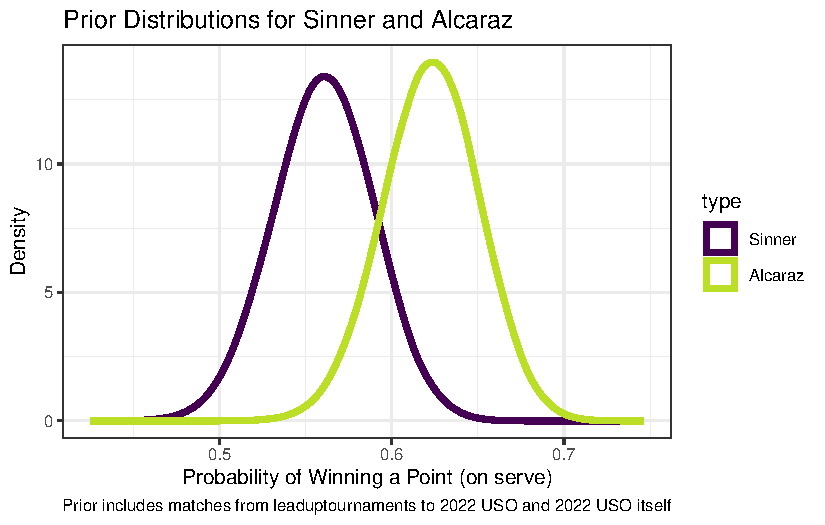
\includegraphics{Project_Write_Up_files/figure-pdf/unnamed-chunk-11-1.pdf}

\linespread{2}

From our prior distributions, we see that Sinner's probability of
winning a point on serve against Alcaraz is centered around 0.57, and
Alcaraz's probability of winning a point on serve against Sinner is
centered around 0.62. These are our starting probability distributions
for the match. Based on their prior matches we have included, we think
that Alcaraz has a higher probability of winning a point on his serve
than Sinner does, but, there is some overlap in their prior
distributions. As each point is played, we update these probability
distributions.

\subsubsection{Prior, Data and
Posterior}\label{prior-data-and-posterior}

Now with our prior distributions for the probabilities that the players
win a point while serving, we can observe how these probabilities update
throughout the match by looking at a specific state of the match.

But first, we need to load in our data for the match between Alcaraz and
Sinner. To do this, we use our function
\texttt{wrangle\_point\_level()}. This function returns a list of two
data frames, and the order is determined by which player is listed as
Player1 and Player2 for the match. The point-level data can be found on
\href{https://github.com/JeffSackmann}{Jeff Sackman's Github} in either
the \texttt{tennis\_atp} or the \texttt{tennis\_wta} repositories. We
can find the match id for the match we are interested in by looking at
the \texttt{atp\_matches\_2022} data frame. We can then use this match
id to load in the point-level data for the match between Alcaraz and
Sinner.

\linespread{0.9}

\begin{Shaded}
\begin{Highlighting}[]
\NormalTok{atp\_matches\_2022 }\OtherTok{\textless{}{-}} \FunctionTok{read\_matches}\NormalTok{(}\StringTok{"atp\_matches\_2022.csv"}\NormalTok{)}
\end{Highlighting}
\end{Shaded}

\linespread{2}

We load in the data for the match between Alcaraz and Sinner using the
match id of \texttt{1503} for their 2022 quarterfinal match:

\linespread{0.9}

\begin{Shaded}
\begin{Highlighting}[]
\DocumentationTok{\#\# returns list of two data frames}
\NormalTok{sin\_alc\_paired }\OtherTok{\textless{}{-}} \FunctionTok{wrangle\_point\_level}\NormalTok{(}\AttributeTok{ext =} \StringTok{"2022{-}usopen{-}points.csv"}\NormalTok{,}
                               \AttributeTok{ID =} \StringTok{"2022{-}usopen{-}1503"}\NormalTok{)}
\DocumentationTok{\#\# first data frame corresponds to player1 (Sinner)}
\NormalTok{sin\_serving }\OtherTok{\textless{}{-}}\NormalTok{ sin\_alc\_paired[[}\DecValTok{1}\NormalTok{]]}
\DocumentationTok{\#\# sescond data frame corresponds to player2 (Alcaraz)}
\NormalTok{alc\_serving }\OtherTok{\textless{}{-}}\NormalTok{ sin\_alc\_paired[[}\DecValTok{2}\NormalTok{]]}
\end{Highlighting}
\end{Shaded}

\linespread{2}

Here we look at a specific state of the match now that we have our data.
For our Alcaraz and Sinner example, we also have their probabilities of
winning a point on serve at the very start of the match. The scoreline
we are looking at for Sinner is when he is serving at 40-15, 1-1 in the
3rd set (a little less than halfway through the match) and see how his
probability of winning a point on serve has changed.

\linespread{0.9}

\begin{Shaded}
\begin{Highlighting}[]
\NormalTok{p1\_serving\_df }\OtherTok{\textless{}{-}}\NormalTok{ sin\_serving }\SpecialCharTok{|\textgreater{}} \FunctionTok{slice}\NormalTok{(}\DecValTok{1}\SpecialCharTok{:}\DecValTok{150}\NormalTok{)}

\NormalTok{p1\_serving\_df }\SpecialCharTok{|\textgreater{}}
  \FunctionTok{summarise}\NormalTok{(}\AttributeTok{points\_won =} \FunctionTok{sum}\NormalTok{(PointWinner }\SpecialCharTok{==} \DecValTok{1}\NormalTok{),}
            \AttributeTok{points\_played =} \FunctionTok{n}\NormalTok{(),}
            \AttributeTok{prop\_won =}\NormalTok{ points\_won }\SpecialCharTok{/}\NormalTok{ points\_played) }\SpecialCharTok{|\textgreater{}}
  \FunctionTok{kable}\NormalTok{()}
\end{Highlighting}
\end{Shaded}

\begin{longtable}[]{@{}rrr@{}}
\toprule\noalign{}
points\_won & points\_played & prop\_won \\
\midrule\noalign{}
\endhead
\bottomrule\noalign{}
\endlastfoot
89 & 150 & 0.5933333 \\
\end{longtable}

\linespread{2}

At this state of the match, Sinner has played 150 points on his serve
and won 89 of them, which is right around 0.6. We'd expect his updated
distribution to shift towards 0.6, as his original probability
distribution was centered around 0.5606.

Now let's plot Sinner's prior distribution with his updated prior
distribution at this specific state of the match.

\linespread{0.9}

\begin{Shaded}
\begin{Highlighting}[]
\DocumentationTok{\#\# get the number of rows in the data frame}
\NormalTok{p1\_niter }\OtherTok{\textless{}{-}}\NormalTok{ p1\_serving\_df }\SpecialCharTok{|\textgreater{}} \FunctionTok{nrow}\NormalTok{()}
\DocumentationTok{\#\# create a storage vector for the probabilities}
\NormalTok{p1\_prob\_store }\OtherTok{\textless{}{-}} \FunctionTok{double}\NormalTok{()}
\DocumentationTok{\#\# create indicator if serving player won the point}
\NormalTok{p1\_serving }\OtherTok{\textless{}{-}}\NormalTok{ p1\_serving\_df }\SpecialCharTok{|\textgreater{}}
    \FunctionTok{mutate}\NormalTok{(}\AttributeTok{server\_won =} \FunctionTok{ifelse}\NormalTok{(PointWinner }\SpecialCharTok{==} \DecValTok{1}\NormalTok{, }\DecValTok{1}\NormalTok{, }\DecValTok{0}\NormalTok{))}
\DocumentationTok{\#\# Use a bayesian generalized linear model to update our prior distribution}
\NormalTok{mod }\OtherTok{\textless{}{-}} \FunctionTok{stan\_glm}\NormalTok{(server\_won }\SpecialCharTok{\textasciitilde{}} \DecValTok{1}\NormalTok{, }\AttributeTok{data =}\NormalTok{ p1\_serving }\SpecialCharTok{|\textgreater{}} \FunctionTok{slice}\NormalTok{(}\DecValTok{1}\SpecialCharTok{:}\NormalTok{p1\_niter),}
                    \AttributeTok{family =}\NormalTok{ binomial,}
                    \AttributeTok{prior\_intercept =} \FunctionTok{normal}\NormalTok{(prior\_sin\_logodds, prior\_sin\_se\_logodds),}
                    \AttributeTok{seed =} \DecValTok{123}\NormalTok{)}
\end{Highlighting}
\end{Shaded}

\linespread{2}

\linespread{0.9}

\begin{Shaded}
\begin{Highlighting}[]
\DocumentationTok{\#\# get the posterior distribution}
\NormalTok{tibble\_mod }\OtherTok{\textless{}{-}} \FunctionTok{as\_tibble}\NormalTok{(mod) }\SpecialCharTok{|\textgreater{}}
  \FunctionTok{mutate}\NormalTok{(}\AttributeTok{prob =} \FunctionTok{expit}\NormalTok{(}\StringTok{\textasciigrave{}}\AttributeTok{(Intercept)}\StringTok{\textasciigrave{}}\NormalTok{)) }\SpecialCharTok{|\textgreater{}}
  \FunctionTok{rename}\NormalTok{(}\AttributeTok{logodds =} \StringTok{\textasciigrave{}}\AttributeTok{(Intercept)}\StringTok{\textasciigrave{}}\NormalTok{)}
\DocumentationTok{\#\# bind tibble\_mod and our prior for sinner, which was created in the chunk plotting}
\DocumentationTok{\#\# both prior distributions for sinner and alcaraz}
\NormalTok{plot\_df }\OtherTok{\textless{}{-}} \FunctionTok{bind\_rows}\NormalTok{(tibble\_mod, prior\_sin\_df, }\AttributeTok{.id =} \StringTok{"type"}\NormalTok{) }\SpecialCharTok{|\textgreater{}}
  \FunctionTok{mutate}\NormalTok{(}\AttributeTok{type =} \FunctionTok{fct\_recode}\NormalTok{(type, }\StringTok{"posterior"} \OtherTok{=} \StringTok{"1"}\NormalTok{,}
                           \StringTok{"prior"} \OtherTok{=} \StringTok{"2"}\NormalTok{),}
         \AttributeTok{type =} \FunctionTok{fct\_relevel}\NormalTok{(type, }\FunctionTok{c}\NormalTok{(}\StringTok{"prior"}\NormalTok{, }\StringTok{"posterior"}\NormalTok{)))}
\DocumentationTok{\#\# plot both the prior and the updated prior}
\FunctionTok{ggplot}\NormalTok{(}\AttributeTok{data =}\NormalTok{ plot\_df, }\FunctionTok{aes}\NormalTok{(}\AttributeTok{x =}\NormalTok{ prob)) }\SpecialCharTok{+}
  \FunctionTok{geom\_density}\NormalTok{(}\FunctionTok{aes}\NormalTok{(}\AttributeTok{linetype =}\NormalTok{ type), }\AttributeTok{adjust =} \DecValTok{2}\NormalTok{,}
               \AttributeTok{linewidth =} \FloatTok{0.9}\NormalTok{) }\SpecialCharTok{+} \DocumentationTok{\#\# adjust smooths it out}
  \FunctionTok{theme\_minimal}\NormalTok{() }\SpecialCharTok{+}
  \FunctionTok{labs}\NormalTok{(}\AttributeTok{title =} \StringTok{"Prior and Posterior Distributions at Specific Match State"}\NormalTok{,}
       \AttributeTok{subtitle =} \StringTok{"Sinner serving at 40{-}15, 1{-}1, 3rd set"}\NormalTok{,}
       \AttributeTok{x =} \StringTok{"Sinner\textquotesingle{}s Probability of Winning a Point (on serve)"}\NormalTok{,}
       \AttributeTok{y =} \StringTok{"Density"}\NormalTok{,}
       \AttributeTok{caption =} \StringTok{"Sinner: 89/150 points won on serve"}\NormalTok{) }\SpecialCharTok{+}
  \FunctionTok{coord\_cartesian}\NormalTok{(}\AttributeTok{ylim =} \FunctionTok{c}\NormalTok{(}\DecValTok{0}\NormalTok{, }\DecValTok{17}\NormalTok{)) }\SpecialCharTok{+}
  \FunctionTok{theme\_bw}\NormalTok{(}\AttributeTok{base\_size =} \DecValTok{10}\NormalTok{)}
\end{Highlighting}
\end{Shaded}

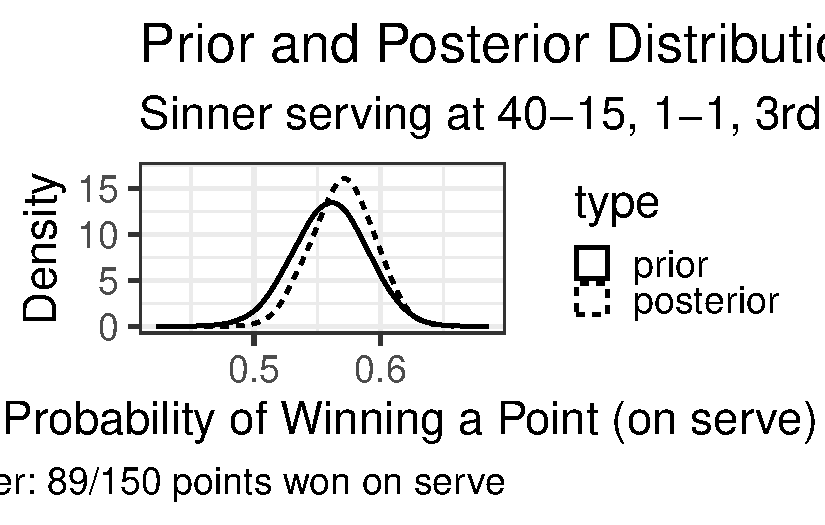
\includegraphics{Project_Write_Up_files/figure-pdf/unnamed-chunk-16-1.pdf}

\linespread{2}

We see that Sinner's probability distribution of winning a point on
serve when he is serving at 40-15, 1-1 in the 3rd set has shifted. As
points are being played, we are getting additional data. That data is
updating the distribution bit by bit. At this point of the match, we
think that Sinner has a slightly higher probability of winning a point
on serve than at the start of the match. With Sinner winnning 89 out of
150 points on serve at this point in the match, it makes sense that his
updated distribution has shifted closer to 0.6. We also see that, as we
obtain additional data in the match, the spread of the distribution
shrinks a little compared to the prior distribution of Sinner's on-serve
point-win probability at the start of the match.

\subsection{Caclulating In-Match-Win
Probability}\label{caclulating-in-match-win-probability}

Now that we have explored how to create the probabilities of winning a
point on serve and seeing how they update throughout the match, we can
use these probabilities to calculate the probability of winning the
match.

\subsubsection{Case Study 1: Alcaraz vs Sinner}\label{sec-alcsin}

With the probability distributions of both players winning a point on
their serve, we can calculate the probability of either player winning
the entire match. We do this by updating the probability distributions
of the players winning a point on serve as each successive point is
played. For a current state of the match, we have the updated
probability distributions of each player winning a point on serve, and
the score at that state of the match. Then, using these updated
point-level probability distributions, we are able to calculate the
overall probability of winning the match.

For our first case study, we continue to use our example that we have
talked through to set up key aspects of this project. We look at the
2022 US Open Quarterfinal match between Jannik Sinner and Carlos
Alcaraz, where Alcaraz defeated Sinner 6-3, 6-7(7), 6-7(0), 7-5, 6-3 in
5 sets.

At the time, this match was highly anticipated to be a close match
between two young, emerging stars in the tennis world. Sinner, an
Italian player, was seeded 11th in the tournament and was known for his
powerful groundstrokes and aggressive playing style. Alcaraz, a Spanish
player, was seeded 3rd in the tournament but had been making waves in
the tennis world with his athleticism and shot-making ability.

With Alcaraz being the eventual match winner, we are exploring the
probability that Alcaraz wins the match.

First, we need to calculate the updated probabilities of Alcaraz and
Sinner winning a point on serve after each successive point is played.
To do this, we use our \texttt{get\_probabilities\_df()} function. This
function takes in the data frames of the players' serving points, the
players' names, the players' original estimated probabilities of winning
a point on serve, and the players' original standard errors (on the
log-odds scale). Before, we looked at Sinner's updated probability
distribution of winning a point on serve at a specific state of the
match. Now, we loop through every single point of the match and obtain
updated probabilities of the two players winning a point on serve after
each successive point. It is worth noting that as Alcaraz serves
multiple points in a row, Sinner's probability of winning a point on
serve does not change as there is no new data we are observing that
would update his probability. Our output is a dataframe that contains
the probabilities of the two players winning a point on serve which is
updated after each successive point.

Note that our original probabilities of winning a point on serve at the
start of the match came from us taking the mean of the log-odds serve
posterior distributions of each player winning a point on serve. We then
converted these log-odds to talk about them in terms of probabilities.

An alternative approach to calculating the probabilities of winning a
point on serve is to take samples from the serve posterior distributions
of the log-odds of winning a point on serve for each player. As we
sample from these distributions, we convert each log-odds sample to a
probability of winning a point on serve. For each sample, we compute the
match-win probability and then average all of these match-win
probabilities to get a final probability of winning the match.

So in our \texttt{get\_probabilities\_df()} function, we save both the
mean log-odds and the distribution centers from sampling in the
dataframe. This allows us to choose which probabilities to use later on,
when we use another function to calculate the overall probability of
winning the match.

\linespread{0.9}

\begin{Shaded}
\begin{Highlighting}[]
\NormalTok{combined\_prob\_sin\_alc\_sp\_df }\OtherTok{\textless{}{-}} \FunctionTok{get\_probabilities\_df}\NormalTok{(}\AttributeTok{p1\_serving\_df =}\NormalTok{ sin\_serving,}
                                 \AttributeTok{p2\_serving\_df =}\NormalTok{ alc\_serving,}
                                 \AttributeTok{p1 =} \StringTok{"Jannik Sinner"}\NormalTok{,}
                                 \AttributeTok{p2 =} \StringTok{"Carlos Alcaraz"}\NormalTok{,}
                                 \AttributeTok{p1\_original\_prob =} \FloatTok{0.2434863}\NormalTok{,}
                                 \AttributeTok{p1\_original\_se =} \FloatTok{0.1193404}\NormalTok{,}
                                 \AttributeTok{p2\_original\_prob =} \FloatTok{0.5017383}\NormalTok{,}
                                 \AttributeTok{p2\_original\_se =} \FloatTok{0.1196950}\NormalTok{)}
\end{Highlighting}
\end{Shaded}

\linespread{2}

We now use the probabilities of the two players winning a point on serve
to calculate the overall probability of the players winning the match.
We simulate the match point by point, updating the probabilities of the
players winning a point on serve as each point is played, and for each
specific state of the match and probabilities of the players winning a
point on serve, we calculate the overall probability of a player winning
the entire match. We use the \texttt{get\_plot\_df()} function to do
this. As noted before the chunk above, we have the option to use the
mean probabilities or the distribution centers from sampling to
calculate the overall probability of winning the match. This is the
\texttt{type} parameter in the function. We set this parameter to
\texttt{"mean"} or \texttt{"distribution"}.

\linespread{0.9}

\begin{Shaded}
\begin{Highlighting}[]
\NormalTok{plot\_sin\_alc\_small\_prior }\OtherTok{\textless{}{-}} \FunctionTok{get\_plot\_df}\NormalTok{(}\AttributeTok{combined\_df =}\NormalTok{ combined\_prob\_sin\_alc\_sp\_df, }
                        \AttributeTok{which\_player\_prob =} \DecValTok{2}\NormalTok{,}
                        \AttributeTok{best\_of\_3 =} \ConstantTok{FALSE}\NormalTok{,}
                        \AttributeTok{advantage =} \ConstantTok{FALSE}\NormalTok{,}
                        \AttributeTok{type =} \StringTok{"distribution"}\NormalTok{) }\SpecialCharTok{|\textgreater{}}
  \FunctionTok{mutate}\NormalTok{(}\AttributeTok{set\_number =} \FunctionTok{as.factor}\NormalTok{(}\FunctionTok{as.numeric}\NormalTok{(total\_sets))) }\SpecialCharTok{|\textgreater{}}
  \DocumentationTok{\#\# fix last row in data set where set\_number is 6, should be a 5}
  \FunctionTok{mutate}\NormalTok{(}\AttributeTok{set\_number =} \FunctionTok{ifelse}\NormalTok{(pt\_number }\SpecialCharTok{==} \FunctionTok{max}\NormalTok{(pt\_number), }\StringTok{\textquotesingle{}5\textquotesingle{}}\NormalTok{, set\_number)) }\SpecialCharTok{|\textgreater{}}
  \FunctionTok{mutate}\NormalTok{(}\AttributeTok{set\_number =} \FunctionTok{as.factor}\NormalTok{(set\_number))}
\end{Highlighting}
\end{Shaded}

\linespread{2}

We can choose how many sets we want to display on our graph, but here we
save colors for up to 5 sets.

\linespread{0.9}

\begin{Shaded}
\begin{Highlighting}[]
\DocumentationTok{\#\# create fills to color sets by}
\NormalTok{fills }\OtherTok{\textless{}{-}} \FunctionTok{c}\NormalTok{(}\StringTok{"\#F57A5C"}\NormalTok{, }\StringTok{"\#F5C25C"}\NormalTok{, }\StringTok{"\#94E25B"}\NormalTok{, }\StringTok{"\#69CEE0"}\NormalTok{, }\StringTok{"\#A875CE"}\NormalTok{)}
\end{Highlighting}
\end{Shaded}

\linespread{2}

We look at just the first set of the match:

\linespread{0.9}

\begin{Shaded}
\begin{Highlighting}[]
\DocumentationTok{\#\# filter for just the first set}
\NormalTok{plot\_first\_set\_sin\_alc }\OtherTok{\textless{}{-}}\NormalTok{ plot\_sin\_alc\_small\_prior }\SpecialCharTok{|\textgreater{}}
  \FunctionTok{filter}\NormalTok{(set\_number }\SpecialCharTok{==} \DecValTok{1}\NormalTok{)}
\DocumentationTok{\#\# create the boundaries for the sets}
\NormalTok{first\_set\_boundaries\_alc\_sin\_small\_prior }\OtherTok{\textless{}{-}}\NormalTok{ plot\_sin\_alc\_small\_prior }\SpecialCharTok{|\textgreater{}}
  \FunctionTok{group\_by}\NormalTok{(set\_number) }\SpecialCharTok{|\textgreater{}}
  \FunctionTok{summarize}\NormalTok{(}\AttributeTok{xmin =} \FunctionTok{min}\NormalTok{(pt\_number) }\SpecialCharTok{{-}} \FloatTok{0.5}\NormalTok{,}
            \AttributeTok{xmax =} \FunctionTok{max}\NormalTok{(pt\_number) }\SpecialCharTok{+} \FloatTok{0.5}\NormalTok{) }\SpecialCharTok{|\textgreater{}}
  \FunctionTok{filter}\NormalTok{(set\_number }\SpecialCharTok{==} \DecValTok{1}\NormalTok{)}
\DocumentationTok{\#\# plot}
\NormalTok{plot\_sin\_alc\_small\_prior }\SpecialCharTok{|\textgreater{}} \FunctionTok{ggplot}\NormalTok{(}\FunctionTok{aes}\NormalTok{(}\AttributeTok{x =}\NormalTok{ pt\_number, }\AttributeTok{y =}\NormalTok{ probability)) }\SpecialCharTok{+}
  \FunctionTok{geom\_rect}\NormalTok{(}\AttributeTok{data =}\NormalTok{ first\_set\_boundaries\_alc\_sin\_small\_prior, }
            \FunctionTok{aes}\NormalTok{(}\AttributeTok{x =} \ConstantTok{NULL}\NormalTok{, }\AttributeTok{y =} \ConstantTok{NULL}\NormalTok{, }\AttributeTok{xmin =}\NormalTok{ xmin, }\AttributeTok{xmax =}\NormalTok{ xmax, }
                \AttributeTok{ymin =} \SpecialCharTok{{-}}\ConstantTok{Inf}\NormalTok{, }\AttributeTok{ymax =} \ConstantTok{Inf}\NormalTok{, }\AttributeTok{fill =}\NormalTok{ set\_number), }\AttributeTok{alpha =} \FloatTok{0.2}\NormalTok{) }\SpecialCharTok{+} 
  \FunctionTok{geom\_line}\NormalTok{(}\AttributeTok{data =}\NormalTok{ plot\_first\_set\_sin\_alc, }\FunctionTok{aes}\NormalTok{(}\AttributeTok{y =}\NormalTok{ win\_prob\_px)) }\SpecialCharTok{+}
  \FunctionTok{labs}\NormalTok{(}\AttributeTok{x =} \StringTok{"Point Number"}\NormalTok{,}
       \AttributeTok{y =} \StringTok{"Probability of Winning Match"}\NormalTok{,}
       \AttributeTok{title =} \StringTok{"Alcaraz vs Sinner US Open Quarterfinal 2022"}\NormalTok{,}
       \AttributeTok{subtitle =} \StringTok{"Probability of Alcaraz Winning Match"}\NormalTok{,}
       \AttributeTok{caption =} \StringTok{"Prior contains \textquotesingle{}lead{-}up\textquotesingle{} tournaments to the 2022 USO and 2022 USO itself"}\NormalTok{,}
       \AttributeTok{color =} \StringTok{"Server"}\NormalTok{) }\SpecialCharTok{+}
  \FunctionTok{coord\_cartesian}\NormalTok{(}\AttributeTok{ylim =} \FunctionTok{c}\NormalTok{(}\DecValTok{0}\NormalTok{, }\DecValTok{1}\NormalTok{),}
                  \AttributeTok{xlim =} \FunctionTok{c}\NormalTok{(}\DecValTok{0}\NormalTok{, }\FunctionTok{nrow}\NormalTok{(plot\_sin\_alc\_small\_prior))) }\SpecialCharTok{+}
  \FunctionTok{scale\_fill\_manual}\NormalTok{(}\AttributeTok{values =}\NormalTok{ fills[}\DecValTok{1}\NormalTok{]) }\SpecialCharTok{+}
  \FunctionTok{theme\_bw}\NormalTok{(}\AttributeTok{base\_size =} \DecValTok{10}\NormalTok{)}
\end{Highlighting}
\end{Shaded}

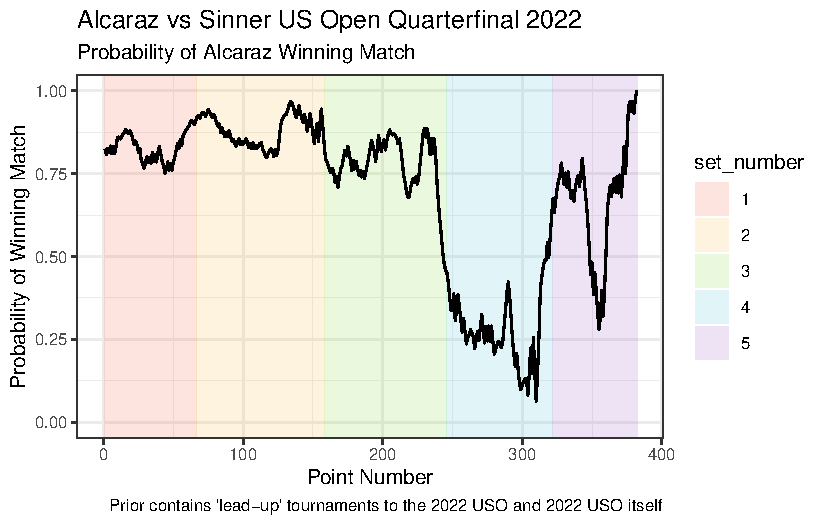
\includegraphics{Project_Write_Up_files/figure-pdf/unnamed-chunk-20-1.pdf}

\linespread{2}

We see Alcaraz start the match with a high probability of winning the
match. This makes sense, as Alcaraz's probability center of winning a
point on serve (0.6228678) is much higher than Sinner's probability
center of winning a point on serve (0.5605726).

Some notable moments in the first set are:

\begin{itemize}
\tightlist
\item
  Alcaraz breaks Sinner's serve in the first game of the match to go up
  1-0.
\item
  Sinner breaks back in the fourth game of the match to even the set at
  2-2, and holds after a long game with many deuce points to go up 3-2.
\item
  Alcaraz then wins the next 4 games in a row to take the first set 6-3,
  so it follows that his probability of winning the match has increased
  since the start of the match.
\item
  Alcaraz's updated probability of winning a point on serve at the end
  of the set is 0.624
\item
  Sinner's updated probability of winning a point on serve at the end of
  the set is 0.549
\end{itemize}

We include all of the sets to plot the entire match:

\linespread{0.9}

\begin{Shaded}
\begin{Highlighting}[]
\DocumentationTok{\#\# not necessary here since we are plotting all sets, but included anyway}
\NormalTok{plot\_five\_sets\_sin\_alc }\OtherTok{\textless{}{-}}\NormalTok{ plot\_sin\_alc\_small\_prior }\SpecialCharTok{|\textgreater{}}
  \FunctionTok{filter}\NormalTok{(set\_number }\SpecialCharTok{==} \DecValTok{1} \SpecialCharTok{|}\NormalTok{ set\_number }\SpecialCharTok{==} \DecValTok{2} \SpecialCharTok{|} 
\NormalTok{           set\_number }\SpecialCharTok{==} \DecValTok{3} \SpecialCharTok{|}\NormalTok{ set\_number }\SpecialCharTok{==} \DecValTok{4} \SpecialCharTok{|} 
\NormalTok{           set\_number }\SpecialCharTok{==} \DecValTok{5}\NormalTok{)}
\DocumentationTok{\#\# create the boundaries for the sets}
\NormalTok{five\_set\_boundaries\_alc\_sin\_small\_prior }\OtherTok{\textless{}{-}}\NormalTok{ plot\_sin\_alc\_small\_prior }\SpecialCharTok{|\textgreater{}}
  \FunctionTok{group\_by}\NormalTok{(set\_number) }\SpecialCharTok{|\textgreater{}}
  \FunctionTok{summarize}\NormalTok{(}\AttributeTok{xmin =} \FunctionTok{min}\NormalTok{(pt\_number) }\SpecialCharTok{{-}} \FloatTok{0.5}\NormalTok{,}
            \AttributeTok{xmax =} \FunctionTok{max}\NormalTok{(pt\_number) }\SpecialCharTok{+} \FloatTok{0.5}\NormalTok{) }\SpecialCharTok{|\textgreater{}}
  \FunctionTok{filter}\NormalTok{(set\_number }\SpecialCharTok{==} \DecValTok{1} \SpecialCharTok{|}\NormalTok{ set\_number }\SpecialCharTok{==} \DecValTok{2} \SpecialCharTok{|} 
\NormalTok{           set\_number }\SpecialCharTok{==} \DecValTok{3} \SpecialCharTok{|}\NormalTok{ set\_number }\SpecialCharTok{==} \DecValTok{4} \SpecialCharTok{|} 
\NormalTok{           set\_number }\SpecialCharTok{==} \DecValTok{5}\NormalTok{)}
\DocumentationTok{\#\# plot}
\NormalTok{plot\_sin\_alc\_small\_prior }\SpecialCharTok{|\textgreater{}} \FunctionTok{ggplot}\NormalTok{(}\FunctionTok{aes}\NormalTok{(}\AttributeTok{x =}\NormalTok{ pt\_number, }\AttributeTok{y =}\NormalTok{ probability)) }\SpecialCharTok{+}
  \FunctionTok{geom\_rect}\NormalTok{(}\AttributeTok{data =}\NormalTok{ five\_set\_boundaries\_alc\_sin\_small\_prior, }
            \FunctionTok{aes}\NormalTok{(}\AttributeTok{x =} \ConstantTok{NULL}\NormalTok{, }\AttributeTok{y =} \ConstantTok{NULL}\NormalTok{, }\AttributeTok{xmin =}\NormalTok{ xmin, }\AttributeTok{xmax =}\NormalTok{ xmax,}
                \AttributeTok{ymin =} \SpecialCharTok{{-}}\ConstantTok{Inf}\NormalTok{, }\AttributeTok{ymax =} \ConstantTok{Inf}\NormalTok{, }\AttributeTok{fill =}\NormalTok{ set\_number), }\AttributeTok{alpha =} \FloatTok{0.2}\NormalTok{) }\SpecialCharTok{+} 
  \FunctionTok{geom\_line}\NormalTok{(}\AttributeTok{data =}\NormalTok{ plot\_five\_sets\_sin\_alc, }\FunctionTok{aes}\NormalTok{(}\AttributeTok{y =}\NormalTok{ win\_prob\_px)) }\SpecialCharTok{+}
  \FunctionTok{labs}\NormalTok{(}\AttributeTok{x =} \StringTok{"Point Number"}\NormalTok{,}
       \AttributeTok{y =} \StringTok{"Probability of Winning Match"}\NormalTok{,}
       \AttributeTok{title =} \StringTok{"Alcaraz vs Sinner US Open Quarterfinal 2022"}\NormalTok{,}
       \AttributeTok{subtitle =} \StringTok{"Probability of Alcaraz Winning Match"}\NormalTok{,}
       \AttributeTok{caption =} \StringTok{"Prior contains \textquotesingle{}lead{-}up\textquotesingle{} tournaments to the 2022 USO and 2022 USO itself"}\NormalTok{,}
       \AttributeTok{color =} \StringTok{"Server"}\NormalTok{) }\SpecialCharTok{+}
  \FunctionTok{coord\_cartesian}\NormalTok{(}\AttributeTok{ylim =} \FunctionTok{c}\NormalTok{(}\DecValTok{0}\NormalTok{, }\DecValTok{1}\NormalTok{),}
                  \AttributeTok{xlim =} \FunctionTok{c}\NormalTok{(}\DecValTok{0}\NormalTok{, }\FunctionTok{nrow}\NormalTok{(plot\_sin\_alc\_small\_prior))) }\SpecialCharTok{+}
  \FunctionTok{scale\_fill\_manual}\NormalTok{(}\AttributeTok{values =}\NormalTok{ fills[}\DecValTok{1}\SpecialCharTok{:}\DecValTok{5}\NormalTok{]) }\SpecialCharTok{+}
  \FunctionTok{theme\_bw}\NormalTok{(}\AttributeTok{base\_size =} \DecValTok{10}\NormalTok{)}
\end{Highlighting}
\end{Shaded}

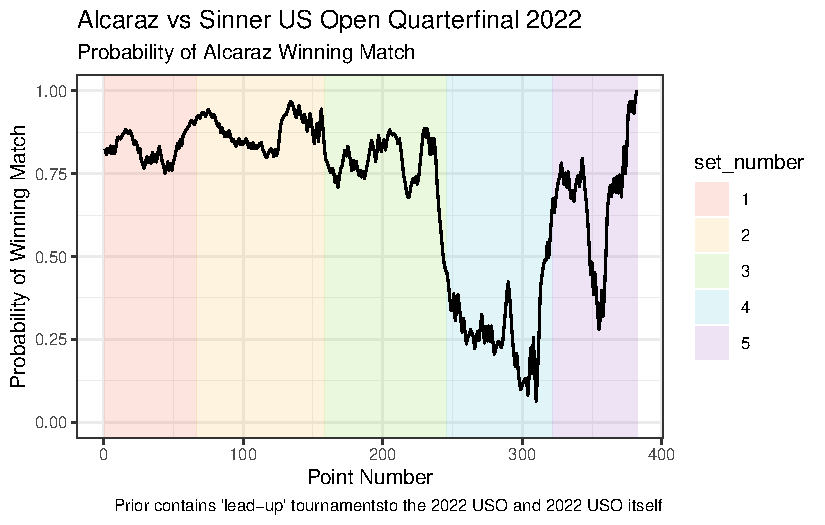
\includegraphics{Project_Write_Up_files/figure-pdf/unnamed-chunk-21-1.pdf}

\linespread{2}

MH: I think you can cut some of the set text below if you want. MH:
Also, all of the point-win probability updates are updates in the
distribution \textbf{center} (or, more specifically, the median
probability).

Second set:

\begin{itemize}
\tightlist
\item
  Sinner breaks early in the set to go up 2-1
\item
  Sinner maintains his break of serve and is serving for the set up 5-3
\item
  Alcaraz breaks back to even the set at 5-5
\item
  Sinner is serving at 5-6, 0-40, and Alcaraz's probability of winning
  the match is very high
\item
  Sinner saves multiple set points and forces a tiebreaker
\item
  Both players save set points in the tiebreaker, but Sinner pulls away
  to win it 9-7
\item
  Alcaraz's updated probability distribution center of winning a point
  on serve at the end of the set is 0.635
\item
  Sinner's updated probability distribution center of winning a point on
  serve at the end of the set is 0.563
\end{itemize}

Third set:

\begin{itemize}
\tightlist
\item
  The set starts with the players trading holds
\item
  Alcaraz breaks serve to go up 3-2
\item
  Alcaraz is serving at 4-3 and Sinner breaks back for 4-4
\item
  At 5-5, Alcaraz breaks Sinner's serve to go up 6-5 serving for the set
\item
  Sinner breaks Alcaraz's serve to force a tiebreaker
\item
  Sinner runs away with the tiebreaker and the set, winning all 7 points
  in a row (7-0)
\item
  Alcaraz's updated probability distribution center of winning a point
  on serve at the end of the set is 0.620
\item
  Sinner's updated probability distribution center of winning a point on
  serve at the end of the set is 0.570
\end{itemize}

Fourth set:

\begin{itemize}
\tightlist
\item
  Sinner breaks Alcaraz's serve in the first game of the set, 1-0
\item
  With Sinner servng at 3-2, Alcaraz breaks back to even the set at 3-3
\item
  Sinner breaks right back to go up 4-3
\item
  Sinner has a match point serving at 5-4, Ad-In, but Alcaraz saves it,
  and breaks for 5-5
\item
  Alcaraz holds for 6-5, and breaks Sinner to win the set 7-5
\item
  Alcaraz's updated probability distribution center of winning a point
  on serve at the end of the set is 0.617
\item
  Sinner's updated probability distribution center of winning a point on
  serve at the end of the set is 0.563
\end{itemize}

Fifth set:

\begin{itemize}
\tightlist
\item
  The players trade holds early
\item
  Sinner breaks Alcaraz's serve to go up 3-2
\item
  Alcaraz breaks right back and then holds to go up 4-3
\item
  Alcaraz breaks again to go up 5-3
\item
  Alcaraz holds to win the set 6-3, and win the overall match
\item
  Alcaraz's updated probability distribution center of winning a point
  on serve at the end of match set is 0.620
\item
  Sinner's updated probability distribution center of winning a point on
  serve at the end of the match is 0.557
\end{itemize}

Observing the dips and peaks in the probability of winning the match as
serves were broken and held, and sets won shows how quickly momentum can
shift in a tennis match. The probability of winning the match is not a
smooth curve, and can change rapidly with the outcome of a few points
because of the scoring system in tennis.

\subsubsection{Changing Prior Distributions}\label{sec-changeprior}

We can change what matches we include in our prior distributions and see
how this affects our probabilities of each player winning a point on
serve at the start of the match. With these different probabilities of
winning a point on serve, we can see how the overall probability of
winning the match changes.

For our example above, we explored the probability of Alcaraz winning
the match against Sinner using matches from the hard court lead-up
tournaments to the 2022 US Open and the 2022 US Open itself to form our
prior distribution. Now, we compare this to two more possible prior
distributions.

We can look at a prior generated that includes all hard court matches
from the 2021 US Open to the quarterfinal round of the 2022 US Open.
This is our ``Large Prior'' distribution that includes more matches than
our original ``Small Prior'' distribution. Due to the larger sample size
of matches, we expect to see smaller changes in the updates of the
probabilities of winning a point on serve throughout the match.

We can also explore what happens if we fix the probabilities of Sinner
and Alcaraz winning a point on serve at a specific value, which we set
at 0.68 for both players (around the tour average). We observe what
happens when we fix this value for the match.

The different priors we choose change the probabilities of winning a
point on serve at the start of the match and thus alter the overall
probability of Alcaraz winning the match. We can see this in the plot
below.

But first, we generate our new priors and calculate the probabilities of
winning a point on serve at the start of the match and update them
accordingly. We start with our ``Large Prior'' distribution and then
move on to the fixed probabilities.

We again use our \texttt{create\_prior()} function to calculate these
values on the log-odds scale.

\linespread{0.9}

\begin{Shaded}
\begin{Highlighting}[]
\NormalTok{aug\_mod\_sin\_large\_prior }\OtherTok{\textless{}{-}} \FunctionTok{create\_prior}\NormalTok{(}\AttributeTok{ext =} \FunctionTok{c}\NormalTok{(}\StringTok{"atp\_matches\_2021.csv"}\NormalTok{,}
                                 \StringTok{"atp\_matches\_2022.csv"}\NormalTok{),}
                         \AttributeTok{tourn\_name =} \StringTok{"Us Open"}\NormalTok{,}
                         \AttributeTok{surf =} \StringTok{"Hard"}\NormalTok{,}
                         \AttributeTok{start\_date =} \StringTok{"2021{-}08{-}30"}\NormalTok{,}
                         \AttributeTok{end\_date =} \StringTok{"2022{-}09{-}06"}\NormalTok{,}
                         \AttributeTok{player1 =} \StringTok{"Jannik Sinner"}\NormalTok{,}
                         \AttributeTok{player2 =} \StringTok{"Carlos Alcaraz"}\NormalTok{,}
                         \AttributeTok{ref\_player =} \StringTok{"Novak Djokovic"}\NormalTok{)}
\NormalTok{aug\_mod\_sin\_large\_prior }\SpecialCharTok{|\textgreater{}} \FunctionTok{kable}\NormalTok{()}
\end{Highlighting}
\end{Shaded}

\linespread{2}

From the output, we see that Sinner has a mean log-odds of winning a
point while serving against Alcaraz of 0.4288085 with a standard error
of 0.0491917, and both of these are on the log odds scale. We can also
see that Sinner has a mean value of winning a point while returning
against Alcaraz of -0.4795682 with a standard error of 0.0497102, and
again both on the log odds scale. To get the log odds of Alcaraz winning
a point while serving against Sinner, we can negate the value of Sinner
winning a point while returning against Alcaraz. We can then convert
these from the log-odds scale to probabilities of winning a point on
serve using the logistic function expit(). The logistic function
transforms the log-odds to probabilities, ensuring that the
probabilities fall within the range {[}0, 1{]}. Note that the standard
error is also smaller than the ``Small Prior'' distribution, as we have
more matches included in our ``Large Prior'' distribution.

\linespread{0.9}

\begin{Shaded}
\begin{Highlighting}[]
\DocumentationTok{\#\# probability Sinner wins a point on serve}
\FunctionTok{expit}\NormalTok{(}\FloatTok{0.4288085}\NormalTok{) }\DocumentationTok{\#\# 0.6055891}
\end{Highlighting}
\end{Shaded}

\begin{verbatim}
[1] 0.6055891
\end{verbatim}

\begin{Shaded}
\begin{Highlighting}[]
\DocumentationTok{\#\# probability Sinner wins a point on return}
\FunctionTok{expit}\NormalTok{(}\SpecialCharTok{{-}}\FloatTok{0.4795682}\NormalTok{) }\DocumentationTok{\#\#  0.3823541}
\end{Highlighting}
\end{Shaded}

\begin{verbatim}
[1] 0.3823541
\end{verbatim}

\begin{Shaded}
\begin{Highlighting}[]
\DocumentationTok{\#\# probability Alcaraz wins a point on serve}
\FunctionTok{expit}\NormalTok{(}\FloatTok{0.4795682}\NormalTok{) }\DocumentationTok{\#\# 0.6176459}
\end{Highlighting}
\end{Shaded}

\begin{verbatim}
[1] 0.6176459
\end{verbatim}

\begin{Shaded}
\begin{Highlighting}[]
\DocumentationTok{\#\# probability Alcaraz wins a point on return}
\FunctionTok{expit}\NormalTok{(}\SpecialCharTok{{-}}\FloatTok{0.4288085}\NormalTok{) }\DocumentationTok{\#\# 0.3944109}
\end{Highlighting}
\end{Shaded}

\begin{verbatim}
[1] 0.3944109
\end{verbatim}

\linespread{2}

Compared to our ``Small Prior'' distribution, we see that the
probabilities of Sinner and Alcaraz winning a point on serve have
changed. From our ``Small Prior'' distribution, Sinner had a probability
centered at 0.5605726 of winning a point on serve, and Alcaraz had a
probability centered at 0.6228678 of winning a point on serve. We have
seen an increase in Sinner's probability, and a decrease in Alcaraz's
probability from that prior to this prior.

We can then calculate the probabilities of them winning a point on their
serve throughout the entire match, updating after each point using our
\texttt{get\_probabilities\_df()} function.

\linespread{0.9}

\begin{Shaded}
\begin{Highlighting}[]
\NormalTok{combined\_prob\_alc\_sin\_lp\_df }\OtherTok{\textless{}{-}} \FunctionTok{get\_probabilities\_df}\NormalTok{(}\AttributeTok{p1\_serving\_df =}\NormalTok{ sin\_serving,}
                                 \AttributeTok{p2\_serving\_df =}\NormalTok{ alc\_serving,}
                                 \AttributeTok{p1 =} \StringTok{"Jannik Sinner"}\NormalTok{,}
                                 \AttributeTok{p2 =} \StringTok{"Carlos Alcaraz"}\NormalTok{,}
                                 \AttributeTok{p1\_original\_prob =} \FloatTok{0.4288085}\NormalTok{,}
                                 \AttributeTok{p1\_original\_se =} \FloatTok{0.04919170}\NormalTok{,}
                                 \AttributeTok{p2\_original\_prob =} \FloatTok{0.4795682}\NormalTok{,}
                                 \AttributeTok{p2\_original\_se =} \FloatTok{0.04971023}\NormalTok{)}
\end{Highlighting}
\end{Shaded}

\linespread{2}

Using the probabilities of the two players winning a point on serve and
the current score of the match as we feed it in, we can calculate the
overall probability of winning the match.

\linespread{0.9}

\begin{Shaded}
\begin{Highlighting}[]
\NormalTok{plot\_sin\_alc\_large\_prior }\OtherTok{\textless{}{-}} \FunctionTok{get\_plot\_df}\NormalTok{(}\AttributeTok{combined\_df =}\NormalTok{ combined\_prob\_alc\_sin\_lp\_df,}
                                        \AttributeTok{which\_player\_prob =} \DecValTok{2}\NormalTok{,}
                                        \AttributeTok{best\_of\_3 =} \ConstantTok{FALSE}\NormalTok{,}
                                        \AttributeTok{advantage =} \ConstantTok{FALSE}\NormalTok{,}
                                        \AttributeTok{type =} \StringTok{"distribution"}\NormalTok{) }\SpecialCharTok{|\textgreater{}}
  \FunctionTok{mutate}\NormalTok{(}\AttributeTok{set\_number =} \FunctionTok{as.factor}\NormalTok{(}\FunctionTok{as.numeric}\NormalTok{(total\_sets))) }\SpecialCharTok{|\textgreater{}}
  \DocumentationTok{\#\# fix last row in data set where set\_number is 6, should be a 5}
  \FunctionTok{mutate}\NormalTok{(}\AttributeTok{set\_number =} \FunctionTok{ifelse}\NormalTok{(pt\_number }\SpecialCharTok{==} \FunctionTok{max}\NormalTok{(pt\_number), }\StringTok{\textquotesingle{}5\textquotesingle{}}\NormalTok{, set\_number)) }\SpecialCharTok{|\textgreater{}}
  \FunctionTok{mutate}\NormalTok{(}\AttributeTok{set\_number =} \FunctionTok{as.factor}\NormalTok{(set\_number))}
\end{Highlighting}
\end{Shaded}

\linespread{2}

Now we have our overall probability of Alcaraz winning the match that
updates after each point is played. We can plot this, but first let's
work through the code to generate the probability of Alcaraz winning the
match when we fix both players' probabilities of winning a point on
serve at 0.68. A lot of the code here is tidied and packed away in
functions that we have used, but we have to do it manually here to input
the 0.68 values for both players.

\linespread{0.9}

\begin{Shaded}
\begin{Highlighting}[]
\NormalTok{sin\_serving\_fp }\OtherTok{\textless{}{-}}\NormalTok{ sin\_serving }\SpecialCharTok{|\textgreater{}} 
  \FunctionTok{mutate}\NormalTok{(}\AttributeTok{player1 =} \StringTok{"Jannik Sinner"}\NormalTok{,}
         \AttributeTok{player2 =} \StringTok{"Carlos Alcaraz"}\NormalTok{) }\SpecialCharTok{|\textgreater{}}
    \DocumentationTok{\#\# also create indicator if serving player won the point}
    \FunctionTok{mutate}\NormalTok{(}\AttributeTok{server\_won =} \FunctionTok{ifelse}\NormalTok{(PointWinner }\SpecialCharTok{==} \DecValTok{1}\NormalTok{, }\DecValTok{1}\NormalTok{, }\DecValTok{0}\NormalTok{))}

\NormalTok{alc\_serving\_fp }\OtherTok{\textless{}{-}}\NormalTok{ alc\_serving }\SpecialCharTok{|\textgreater{}} 
  \FunctionTok{mutate}\NormalTok{(}\AttributeTok{player1 =} \StringTok{"Jannik Sinner"}\NormalTok{,}
         \AttributeTok{player2 =} \StringTok{"Carlos Alcaraz"}\NormalTok{) }\SpecialCharTok{|\textgreater{}}
    \DocumentationTok{\#\# also create indicator if serving player won the point}
    \FunctionTok{mutate}\NormalTok{(}\AttributeTok{server\_won =} \FunctionTok{ifelse}\NormalTok{(PointWinner }\SpecialCharTok{==} \DecValTok{2}\NormalTok{, }\DecValTok{1}\NormalTok{, }\DecValTok{0}\NormalTok{))}

\NormalTok{combined\_sin\_alc\_fixed\_df }\OtherTok{\textless{}{-}} \FunctionTok{bind\_rows}\NormalTok{(sin\_serving\_fp, alc\_serving\_fp) }\SpecialCharTok{|\textgreater{}}
    \FunctionTok{arrange}\NormalTok{(pt\_number) }\SpecialCharTok{|\textgreater{}}
  \FunctionTok{mutate}\NormalTok{(}\AttributeTok{p1\_wserv\_prob =} \FloatTok{0.68}\NormalTok{,}
         \AttributeTok{p2\_wserv\_prob =} \FloatTok{0.68}\NormalTok{) }\SpecialCharTok{|\textgreater{}}
  \FunctionTok{mutate}\NormalTok{(}\AttributeTok{P1SetsWon =} \FunctionTok{cumsum}\NormalTok{(SetWinner }\SpecialCharTok{==} \DecValTok{1}\NormalTok{),}
           \AttributeTok{P2SetsWon =} \FunctionTok{cumsum}\NormalTok{(SetWinner }\SpecialCharTok{==} \DecValTok{2}\NormalTok{)) }\SpecialCharTok{|\textgreater{}}
  \FunctionTok{select}\NormalTok{(pt\_number, player1, player2, PointServer, p1\_wserv\_prob, p2\_wserv\_prob,}
\NormalTok{         P1PointsWon, P2PointsWon, P1GamesWon, P2GamesWon, P1SetsWon, P2SetsWon) }\SpecialCharTok{|\textgreater{}}
  \FunctionTok{mutate}\NormalTok{(}\AttributeTok{PointServer =} \FunctionTok{case\_when}\NormalTok{(P1PointsWon }\SpecialCharTok{==} \DecValTok{0} \SpecialCharTok{\&} 
\NormalTok{                                   P2PointsWon }\SpecialCharTok{==} \DecValTok{0} \SpecialCharTok{\&} 
\NormalTok{                                   PointServer }\SpecialCharTok{==} \DecValTok{1} \SpecialCharTok{\textasciitilde{}} \DecValTok{2}\NormalTok{,}
\NormalTok{                                 P1PointsWon }\SpecialCharTok{==} \DecValTok{0} \SpecialCharTok{\&} 
\NormalTok{                                   P2PointsWon }\SpecialCharTok{==} \DecValTok{0} \SpecialCharTok{\&} 
\NormalTok{                                   PointServer }\SpecialCharTok{==} \DecValTok{2} \SpecialCharTok{\textasciitilde{}} \DecValTok{1}\NormalTok{,}
                                 \ConstantTok{TRUE} \SpecialCharTok{\textasciitilde{}}\NormalTok{ PointServer))}

\NormalTok{plot\_sin\_alc\_fixed\_prior }\OtherTok{\textless{}{-}} \FunctionTok{get\_plot\_df}\NormalTok{(}\AttributeTok{combined\_df =}\NormalTok{ combined\_sin\_alc\_fixed\_df, }
                        \AttributeTok{which\_player\_prob =} \DecValTok{2}\NormalTok{,}
                        \AttributeTok{best\_of\_3 =} \ConstantTok{FALSE}\NormalTok{,}
                        \AttributeTok{advantage =} \ConstantTok{FALSE}\NormalTok{,}
                        \AttributeTok{type =} \StringTok{"mean"}\NormalTok{) }\SpecialCharTok{|\textgreater{}}
  \FunctionTok{mutate}\NormalTok{(}\AttributeTok{set\_number =} \FunctionTok{as.factor}\NormalTok{(}\FunctionTok{as.numeric}\NormalTok{(total\_sets))) }\SpecialCharTok{|\textgreater{}}
  \DocumentationTok{\#\# fix last row in data set where set\_number is 6, should be a 5}
  \FunctionTok{mutate}\NormalTok{(}\AttributeTok{set\_number =} \FunctionTok{ifelse}\NormalTok{(pt\_number }\SpecialCharTok{==} \FunctionTok{max}\NormalTok{(pt\_number), }\StringTok{\textquotesingle{}5\textquotesingle{}}\NormalTok{, set\_number)) }\SpecialCharTok{|\textgreater{}}
  \FunctionTok{mutate}\NormalTok{(}\AttributeTok{set\_number =} \FunctionTok{as.factor}\NormalTok{(set\_number))}
\end{Highlighting}
\end{Shaded}

\linespread{2}

And now that we have the probabilities of Alcaraz winning the match with
our ``Small Prior'', ``Large Prior'', and the fixed probability of both
Sinner and Alcaraz winning a point on serve set at 0.68, we can plot
these alongside one another.

\linespread{0.9}

\begin{Shaded}
\begin{Highlighting}[]
\NormalTok{plot\_sin\_alc\_small\_prior }\SpecialCharTok{|\textgreater{}} \FunctionTok{ggplot}\NormalTok{(}\FunctionTok{aes}\NormalTok{(}\AttributeTok{x =}\NormalTok{ pt\_number, }\AttributeTok{y =}\NormalTok{ probability)) }\SpecialCharTok{+}
  \FunctionTok{geom\_line}\NormalTok{(}\FunctionTok{aes}\NormalTok{(}\AttributeTok{y =}\NormalTok{ win\_prob\_px, }
                \AttributeTok{color =} \FunctionTok{factor}\NormalTok{(}\StringTok{"Small Prior"}\NormalTok{, }
                               \AttributeTok{levels =} \FunctionTok{c}\NormalTok{(}\StringTok{"Small Prior"}\NormalTok{, }
                                          \StringTok{"Large Prior"}\NormalTok{, }
                                          \StringTok{"Fixed Probability"}\NormalTok{))), }
                \AttributeTok{alpha =} \FloatTok{0.9}\NormalTok{) }\SpecialCharTok{+}
  \FunctionTok{geom\_line}\NormalTok{(}\AttributeTok{data =}\NormalTok{ plot\_sin\_alc\_large\_prior, }
            \FunctionTok{aes}\NormalTok{(}\AttributeTok{y =}\NormalTok{ win\_prob\_px, }\AttributeTok{color =} \StringTok{"Large Prior"}\NormalTok{), }\AttributeTok{alpha =} \FloatTok{0.5}\NormalTok{) }\SpecialCharTok{+}
  \FunctionTok{geom\_line}\NormalTok{(}\AttributeTok{data =}\NormalTok{ plot\_sin\_alc\_fixed\_prior, }
            \FunctionTok{aes}\NormalTok{(}\AttributeTok{y =}\NormalTok{ win\_prob\_px, }
                \AttributeTok{color =} \StringTok{"Fixed Probability (0.68)"}\NormalTok{), }
            \AttributeTok{alpha =} \FloatTok{0.5}\NormalTok{) }\SpecialCharTok{+}
  \FunctionTok{labs}\NormalTok{(}\AttributeTok{x =} \StringTok{"Point Number"}\NormalTok{,}
       \AttributeTok{y =} \StringTok{"Probability of Winning Match"}\NormalTok{,}
       \AttributeTok{title =} \StringTok{"Alcaraz vs Sinner US Open Quarterfinal 2022"}\NormalTok{,}
       \AttributeTok{subtitle =} \StringTok{"Probability of Alcaraz Winning Match with Different Priors"}\NormalTok{,}
       \AttributeTok{caption =} \StringTok{"Comparing Different Prior Distributions"}\NormalTok{,}
       \AttributeTok{color =} \StringTok{"Server"}\NormalTok{) }\SpecialCharTok{+}
  \FunctionTok{scale\_color\_manual}\NormalTok{(}\AttributeTok{values =} \FunctionTok{c}\NormalTok{(}\StringTok{"Small Prior"} \OtherTok{=} \StringTok{"red"}\NormalTok{, }
                                \StringTok{"Large Prior"} \OtherTok{=} \StringTok{"blue"}\NormalTok{, }
                                \StringTok{"Fixed Probability"} \OtherTok{=} \StringTok{"green"}\NormalTok{),}
                     \AttributeTok{labels =} \FunctionTok{c}\NormalTok{(}\StringTok{"Small Prior"}\NormalTok{, }
                                \StringTok{"Large Prior"}\NormalTok{, }
                                \StringTok{"Fixed Probability (0.68)"}\NormalTok{)) }\SpecialCharTok{+}
  \FunctionTok{coord\_cartesian}\NormalTok{(}\AttributeTok{ylim =} \FunctionTok{c}\NormalTok{(}\DecValTok{0}\NormalTok{, }\DecValTok{1}\NormalTok{),}
                  \AttributeTok{xlim =} \FunctionTok{c}\NormalTok{(}\DecValTok{0}\NormalTok{, }\FunctionTok{nrow}\NormalTok{(plot\_sin\_alc\_small\_prior))) }\SpecialCharTok{+}
  \FunctionTok{scale\_colour\_viridis\_d}\NormalTok{(}\AttributeTok{end =} \FloatTok{0.9}\NormalTok{) }\SpecialCharTok{+}
  \FunctionTok{theme\_bw}\NormalTok{(}\AttributeTok{base\_size =} \DecValTok{10}\NormalTok{) }\SpecialCharTok{+}
  \FunctionTok{annotate}\NormalTok{(}\StringTok{"text"}\NormalTok{, }\AttributeTok{x =} \DecValTok{110}\NormalTok{, }\AttributeTok{y =} \FloatTok{0.2}\NormalTok{, }
           \AttributeTok{label =} \StringTok{"Starting Win{-}Serve Probabilities:"}\NormalTok{, }
           \AttributeTok{size =} \FloatTok{3.5}\NormalTok{, }\AttributeTok{color =} \StringTok{"black"}\NormalTok{) }\SpecialCharTok{+}
  \FunctionTok{annotate}\NormalTok{(}\StringTok{"text"}\NormalTok{, }\AttributeTok{x =} \DecValTok{110}\NormalTok{, }\AttributeTok{y =} \FloatTok{0.15}\NormalTok{, }
           \AttributeTok{label =} \FunctionTok{paste0}\NormalTok{(}
             \StringTok{"\textquotesingle{}Small Prior {-} \textquotesingle{}*p[alcaraz]: 0.6229*\textquotesingle{}, \textquotesingle{}*p[sinner]: 0.5606"}\NormalTok{), }
           \AttributeTok{size =} \FloatTok{3.5}\NormalTok{, }\AttributeTok{color =} \StringTok{"black"}\NormalTok{, }\AttributeTok{parse =} \ConstantTok{TRUE}\NormalTok{) }\SpecialCharTok{+}
  \FunctionTok{annotate}\NormalTok{(}\StringTok{"text"}\NormalTok{, }\AttributeTok{x =} \DecValTok{110}\NormalTok{, }\AttributeTok{y =} \FloatTok{0.1}\NormalTok{, }
           \AttributeTok{label =} \FunctionTok{paste0}\NormalTok{(}
             \StringTok{"\textquotesingle{}Large Prior {-} \textquotesingle{}*p[alcaraz]: 0.61768*\textquotesingle{}, \textquotesingle{}*p[sinner]: 0.6056"}\NormalTok{), }
           \AttributeTok{size =} \FloatTok{3.5}\NormalTok{, }\AttributeTok{color =} \StringTok{"black"}\NormalTok{, }\AttributeTok{parse =} \ConstantTok{TRUE}\NormalTok{) }\SpecialCharTok{+}
  \FunctionTok{annotate}\NormalTok{(}\StringTok{"text"}\NormalTok{, }\AttributeTok{x =} \DecValTok{110}\NormalTok{, }\AttributeTok{y =} \FloatTok{0.05}\NormalTok{, }
           \AttributeTok{label =} \StringTok{"\textquotesingle{}Fixed Probability {-} \textquotesingle{}*p[alcaraz]: 0.68*\textquotesingle{}, \textquotesingle{}*p[sinner]: 0.68"}\NormalTok{, }
           \AttributeTok{size =} \FloatTok{3.5}\NormalTok{, }\AttributeTok{color =} \StringTok{"black"}\NormalTok{, }\AttributeTok{parse =} \ConstantTok{TRUE}\NormalTok{)}
\end{Highlighting}
\end{Shaded}

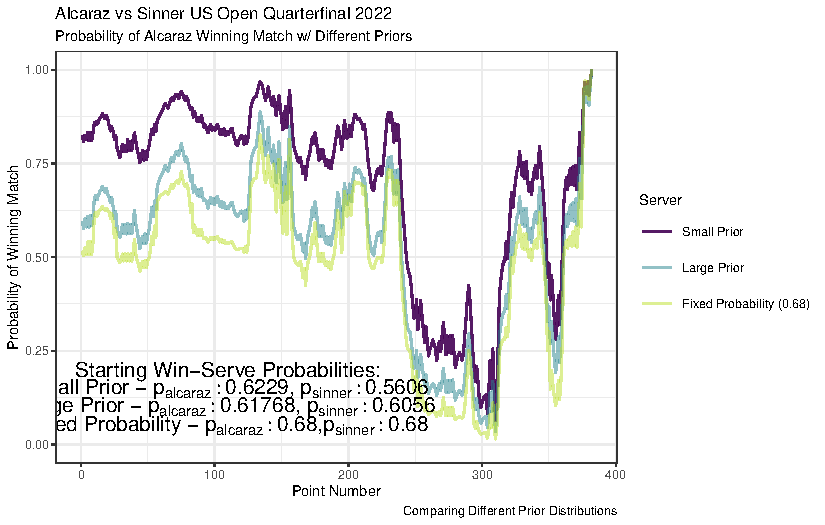
\includegraphics{Project_Write_Up_files/figure-pdf/unnamed-chunk-27-1.pdf}

\linespread{2}

We can see here now that using different priors changes the
probabilities of Alcaraz and Sinner winning a point on their serve at
the start of the match, and lead to different probabilities of Alcaraz
winning the overall match. The different probabilities of winning a
point at the start of the match for the different players are shown in
the annotations on the bottom left of the plot.

The prior we originally looked at for this match is the purple line
labeled ``Small Prior''. In the ``Small Prior'' we included leadup
tournaments to the 2022 US Open and the early rounds of the 2022 US Open
to calculate the probabilities of Sinner and Alcaraz winning a point on
their serve. We see that this line starts with the highest probability
of Alcaraz winning the match, due to this prior generating probabilities
of winning a point on serve between the two players that had the
greatest difference between them (in favor of Alcaraz).

In the ``Large Prior'', the blueish line, we are including all hard
court matches over the last year including the 2021 US Open, and early
rounds of the 2022 US Open. The probabilities of winning a point on
serve for the two players are closer together in this prior, and we see
that the probability of Alcaraz winning the match is lower at the start
of the match compared to the ``Small Prior''.

We can also see what happens when we fix both of their probabilities of
winning a point on serve at 0.68, and this is the yellow line here. The
probability of Alcaraz winning the match starts at 0.5, as we would
expect, due to both players having the same probability of winning a
point on serve.

We can see the changes in the probability of Alcaraz winning the match
based on these different starting probabilities of winning a point on
serve, which we generated using different prior distributions.

\subsubsection{Case Study 2: Gauff vs Sabalenka}\label{sec-gauffsab}

While we have focused on the Alcaraz-Sinner match in the 2022 U.S. Open,
we can apply the methods described above to any match with available
point-level data, including matches on the women's tour. For our second
case study, we look at the 2023 US Open Women's Singles Final match
between Coco Gauff and Arnya Sabalenka.

Gauff, a young, rising American star was looking for her first Grand
Slam title at the age of 19. Sabalenka, a powerful Belarusian player,
was looking for her second Grand Slam title, winning the Australian Open
back in January of that year. Gauff came into the tournament on a very
hot streak, having won lead-up tournaments in Washington, D.C. and
Cincinnati. The win in D.C. was her first at the WTA 500 level, and in
Cincinnati her first at the Masters 1000 level.

Gauff was able to come from behind and win in 3 sets: 2-6, 6-3, 6-2, and
capture her first Grand Slam title.

In women's tennis, breaks of serve are more common. This is because
women are often better returners, and often generate less of an
advantage when serving. On the men's side we saw big spikes for breaking
serve on the plot of in-match-win probability. On the women's side, we
expect to see some jumps for both breaks and holds, but, we would expect
that the jumps are less extreme in general.

With Gauff winning the match, we are exploring the probability that
Gauff wins the match.

First, we need to calculate the probability of Gauff winning a point
while serving against Sabalenka and the probability of Sabalenka winning
a point while serving against Gauff. We use our \texttt{create\_prior()}
function again, and use a similar prior from the exploration of the
match between Sinner and Alcaraz. For the prior, we include matches in
the hard court lead-up tournaments to the 2023 Women's US Open and the
earlier rounds of the 2023 US Open before the final was played.

\linespread{0.9}

\begin{Shaded}
\begin{Highlighting}[]
\NormalTok{aug\_mod\_gau\_small\_prior }\OtherTok{\textless{}{-}} \FunctionTok{create\_prior}\NormalTok{(}\AttributeTok{ext =} \StringTok{"wta\_matches\_2023.csv"}\NormalTok{,}
                         \AttributeTok{tourn\_name =} \StringTok{"Us Open"}\NormalTok{,}
                         \AttributeTok{surf =} \StringTok{"Hard"}\NormalTok{,}
                         \AttributeTok{start\_date =} \StringTok{"2023{-}07{-}24"}\NormalTok{,}
                         \AttributeTok{end\_date =} \StringTok{"2023{-}09{-}8"}\NormalTok{,}
                         \AttributeTok{player1 =} \StringTok{"Coco Gauff"}\NormalTok{,}
                         \AttributeTok{player2 =} \StringTok{"Aryna Sabalenka"}\NormalTok{,}
                         \AttributeTok{ref\_player =} \StringTok{"Iga Swiatek"}\NormalTok{)}
\NormalTok{aug\_mod\_gau\_small\_prior }\SpecialCharTok{|\textgreater{}} \FunctionTok{kable}\NormalTok{()}
\end{Highlighting}
\end{Shaded}

\linespread{2}

From the output, we see that Gauff has a mean value of winning a point
while serving against Sabalenka of \texttt{0.3555439} with a standard
error of \texttt{0.1026245}, and both of these are on the log-odds
scale. We can also see that Gauff has a mean value of winning a point
while returning against Sabalenka of \texttt{-0.1906711} with a standard
error of \texttt{0.1049427}. We can negate the value of Gauff winning a
point while returning against Sabalenka to get Sabalenka's probability
of winning a point while serving against Gauff. We can then convert
these from the log-odds scale to probabilities of winning a point on
serve using the logistic function \texttt{expit()}.

\linespread{0.9}

\begin{Shaded}
\begin{Highlighting}[]
\DocumentationTok{\#\# probability Gauff wins a point on serve}
\FunctionTok{expit}\NormalTok{(}\FloatTok{0.3555439}\NormalTok{) }\DocumentationTok{\#\# 0.5879613}
\end{Highlighting}
\end{Shaded}

\begin{verbatim}
[1] 0.5879613
\end{verbatim}

\begin{Shaded}
\begin{Highlighting}[]
\DocumentationTok{\#\# probability Gauff wins a point on return}
\FunctionTok{expit}\NormalTok{(}\SpecialCharTok{{-}}\FloatTok{0.1906711}\NormalTok{) }\DocumentationTok{\#\# 0.4524761}
\end{Highlighting}
\end{Shaded}

\begin{verbatim}
[1] 0.4524761
\end{verbatim}

\begin{Shaded}
\begin{Highlighting}[]
\DocumentationTok{\#\# probability Sabalenka wins a point on serve}
\FunctionTok{expit}\NormalTok{(}\FloatTok{0.1906711}\NormalTok{) }\DocumentationTok{\#\# 0.5475239}
\end{Highlighting}
\end{Shaded}

\begin{verbatim}
[1] 0.5475239
\end{verbatim}

\begin{Shaded}
\begin{Highlighting}[]
\DocumentationTok{\#\# probability Sabalenka wins a point on return}
\FunctionTok{expit}\NormalTok{(}\SpecialCharTok{{-}}\FloatTok{0.3555439}\NormalTok{) }\DocumentationTok{\#\# 0.4120387}
\end{Highlighting}
\end{Shaded}

\begin{verbatim}
[1] 0.4120387
\end{verbatim}

\linespread{2}

We can load in our point-level data for the match with our function
\texttt{wrangle\_point\_level()}.

\linespread{0.9}

\begin{Shaded}
\begin{Highlighting}[]
\DocumentationTok{\#\# returns list of two data frames}
\NormalTok{both\_gauff\_saba\_serving\_df }\OtherTok{\textless{}{-}} \FunctionTok{wrangle\_point\_level}\NormalTok{(}\AttributeTok{ext =} \StringTok{"2023{-}usopen{-}points.csv"}\NormalTok{,}
                               \AttributeTok{ID =} \StringTok{"2023{-}usopen{-}2701"}\NormalTok{)}
\DocumentationTok{\#\# first data frame corresponds to player1 (Gauff)}
\NormalTok{gauff\_serving }\OtherTok{\textless{}{-}}\NormalTok{ both\_gauff\_saba\_serving\_df[[}\DecValTok{1}\NormalTok{]]}
\DocumentationTok{\#\# second data frame corresponds to player2 (Sabalenka)}
\NormalTok{saba\_serving }\OtherTok{\textless{}{-}}\NormalTok{ both\_gauff\_saba\_serving\_df[[}\DecValTok{2}\NormalTok{]]}
\end{Highlighting}
\end{Shaded}

\linespread{2}

We use the \texttt{get\_probabilities\_df()} function to calculate the
updated probabilities of Gauff and Sabalenka winning a point on serve
after each successive point is played.

\linespread{0.9}

\begin{Shaded}
\begin{Highlighting}[]
\NormalTok{combined\_prob\_gauff\_sab\_sp\_df }\OtherTok{\textless{}{-}} \FunctionTok{get\_probabilities\_df}\NormalTok{(}\AttributeTok{p1\_serving\_df =}\NormalTok{ gauff\_serving,}
                                 \AttributeTok{p2\_serving\_df =}\NormalTok{ saba\_serving,}
                                 \AttributeTok{p1 =} \StringTok{"Coco Gauff"}\NormalTok{,}
                                 \AttributeTok{p2 =} \StringTok{"Aryna Sabalenka"}\NormalTok{,}
                                 \AttributeTok{p1\_original\_prob =} \FloatTok{0.3555439}\NormalTok{,}
                                 \AttributeTok{p1\_original\_se =} \FloatTok{0.1026245}\NormalTok{,}
                                 \AttributeTok{p2\_original\_prob =} \FloatTok{0.1906711}\NormalTok{,}
                                 \AttributeTok{p2\_original\_se =} \FloatTok{0.1049427}\NormalTok{)}
\end{Highlighting}
\end{Shaded}

\linespread{2}

With the probabilities of the Gauff and Sabalenka winning a point on
serve updated for the entire match, we can calculate the overall
probability of the Gauff winning the match. We use the
\texttt{get\_plot\_df()} function to do this.

\linespread{0.9}

\begin{Shaded}
\begin{Highlighting}[]
\NormalTok{plot\_gauff\_sab\_small\_prior }\OtherTok{\textless{}{-}} \FunctionTok{get\_plot\_df}\NormalTok{(}\AttributeTok{combined\_df =}\NormalTok{ combined\_prob\_gauff\_sab\_sp\_df,}
                                        \AttributeTok{which\_player\_prob =} \DecValTok{1}\NormalTok{,}
                                        \AttributeTok{best\_of\_3 =} \ConstantTok{TRUE}\NormalTok{,}
                                        \AttributeTok{advantage =} \ConstantTok{FALSE}\NormalTok{,}
                                        \AttributeTok{type =} \StringTok{"distribution"}\NormalTok{) }\SpecialCharTok{|\textgreater{}}
  \FunctionTok{mutate}\NormalTok{(}\AttributeTok{set\_number =} \FunctionTok{as.factor}\NormalTok{(}\FunctionTok{as.numeric}\NormalTok{(total\_sets))) }\SpecialCharTok{|\textgreater{}}
  \DocumentationTok{\#\# fix last row in data set where set\_number is 4, should be a 3}
  \FunctionTok{mutate}\NormalTok{(}\AttributeTok{set\_number =} \FunctionTok{ifelse}\NormalTok{(pt\_number }\SpecialCharTok{==} \FunctionTok{max}\NormalTok{(pt\_number), }\StringTok{\textquotesingle{}3\textquotesingle{}}\NormalTok{, set\_number)) }\SpecialCharTok{|\textgreater{}}
  \FunctionTok{mutate}\NormalTok{(}\AttributeTok{set\_number =} \FunctionTok{as.factor}\NormalTok{(set\_number))}
\end{Highlighting}
\end{Shaded}

\linespread{2}

And now we can plot the probability of Gauff winning the match:

\linespread{0.9}

\begin{Shaded}
\begin{Highlighting}[]
\DocumentationTok{\#\# create the boundaries for the sets}
\NormalTok{set\_boundaries\_gauff\_sab\_small\_prior }\OtherTok{\textless{}{-}}\NormalTok{ plot\_gauff\_sab\_small\_prior }\SpecialCharTok{|\textgreater{}}
  \FunctionTok{group\_by}\NormalTok{(set\_number) }\SpecialCharTok{|\textgreater{}}
  \FunctionTok{summarize}\NormalTok{(}\AttributeTok{xmin =} \FunctionTok{min}\NormalTok{(pt\_number) }\SpecialCharTok{{-}} \FloatTok{0.5}\NormalTok{,}
            \AttributeTok{xmax =} \FunctionTok{max}\NormalTok{(pt\_number) }\SpecialCharTok{+} \FloatTok{0.5}\NormalTok{)}
\DocumentationTok{\#\# plot}
\NormalTok{plot\_gauff\_sab\_small\_prior }\SpecialCharTok{|\textgreater{}} \FunctionTok{ggplot}\NormalTok{(}\FunctionTok{aes}\NormalTok{(}\AttributeTok{x =}\NormalTok{ pt\_number, }\AttributeTok{y =}\NormalTok{ probability)) }\SpecialCharTok{+}
  \FunctionTok{geom\_rect}\NormalTok{(}\AttributeTok{data =}\NormalTok{ set\_boundaries\_gauff\_sab\_small\_prior, }
            \FunctionTok{aes}\NormalTok{(}\AttributeTok{x =} \ConstantTok{NULL}\NormalTok{, }\AttributeTok{y =} \ConstantTok{NULL}\NormalTok{, }\AttributeTok{xmin =}\NormalTok{ xmin, }\AttributeTok{xmax =}\NormalTok{ xmax, }
                \AttributeTok{ymin =} \SpecialCharTok{{-}}\ConstantTok{Inf}\NormalTok{, }\AttributeTok{ymax =} \ConstantTok{Inf}\NormalTok{, }\AttributeTok{fill =}\NormalTok{ set\_number), }\AttributeTok{alpha =} \FloatTok{0.2}\NormalTok{) }\SpecialCharTok{+} 
  \FunctionTok{geom\_line}\NormalTok{(}\FunctionTok{aes}\NormalTok{(}\AttributeTok{y =}\NormalTok{ win\_prob\_px)) }\SpecialCharTok{+}
  \FunctionTok{labs}\NormalTok{(}\AttributeTok{x =} \StringTok{"Point Number"}\NormalTok{,}
       \AttributeTok{y =} \StringTok{"Probability of Winning Match"}\NormalTok{,}
       \AttributeTok{title =} \StringTok{"Gauff vs Sabalenka US Open Final 2023"}\NormalTok{,}
       \AttributeTok{subtitle =} \StringTok{"Probability of Gauff Winning Match"}\NormalTok{,}
       \AttributeTok{caption =} \StringTok{"Prior contains \textquotesingle{}lead{-}up\textquotesingle{} tournaments to the 2023 USO and 2023 USO itself"}\NormalTok{,}
       \AttributeTok{color =} \StringTok{"Server"}\NormalTok{) }\SpecialCharTok{+}
  \FunctionTok{coord\_cartesian}\NormalTok{(}\AttributeTok{ylim =} \FunctionTok{c}\NormalTok{(}\DecValTok{0}\NormalTok{, }\ConstantTok{NA}\NormalTok{)) }\SpecialCharTok{+}
  \FunctionTok{theme\_bw}\NormalTok{()}
\end{Highlighting}
\end{Shaded}

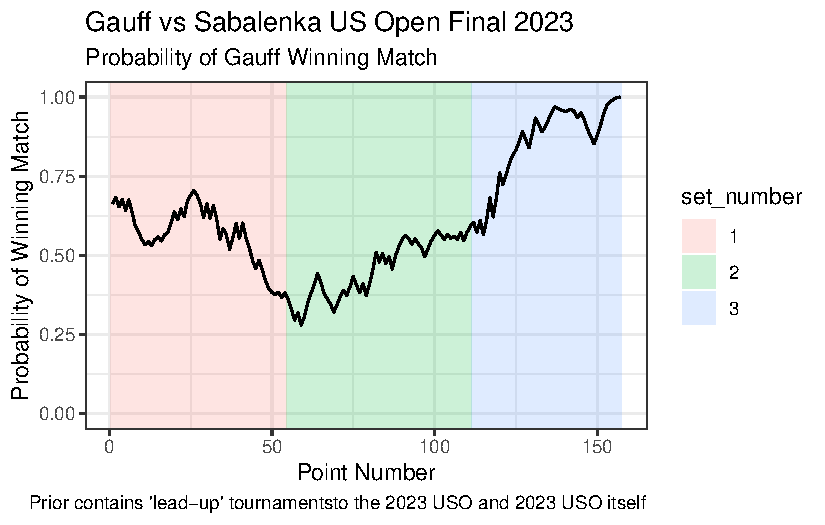
\includegraphics{Project_Write_Up_files/figure-pdf/unnamed-chunk-33-1.pdf}

\linespread{2}

We see Gauff start with a high probability of winning the match (above
0.5) due to her probability of winning a point on serve being higher
than Sabalenka's at the beginning of the match.

First set:

\begin{itemize}
\tightlist
\item
  Sabalenka starts off hot and breaks Gauff's serve in the first game of
  the match
\item
  With Sabalenka serving at 2-1, Gauff breaks back to level the set at
  2-2
\item
  Sabalenka wins the next 4 games to take the first set 6-2
\item
  Gauff's updated probability distribution center of winning a point on
  serve at the end of the set is 0.578
\item
  Sabalenkas' updated probability distribution center of winning a point
  on serve at the end of the set is 0.552
\end{itemize}

We see Gauff's probability of winning the match drop significantly after
this first set.

Second set:

\begin{itemize}
\tightlist
\item
  Gauff saves multiple break points in the first game and is able to
  hold for 1-0
\item
  Gauff breaks Sabalenka's serve in the fourth game of the set to go up
  3-1
\item
  Gauff is able to maintain her break of serve and take the second set
  6-3
\item
  Gauff's updated probability distribution center of winning a point on
  serve at the end of the set is 0.585
\item
  Sabalenkas' updated probability distribution center of winning a point
  on serve at the end of the set is 0.554
\end{itemize}

Third set:

\begin{itemize}
\tightlist
\item
  Gauff breaks Sabalenka's serve in the first game of the set
\item
  Gauff holds for 2-0
\item
  Gauff breaks Sabalenka's serve again in the third game of the set
\item
  Gauff holds for 4-0
\item
  Sabalenka slows Gauff's momentum as she holds for 1-4
\item
  Sabalenka breaks Gauff's serve, 2-4
\item
  Gauff breaks right back to go up 5-2, and serves out the match to win
  6-2
\item
  Gauff's updated probability distribution center of winning a point on
  serve at the end of the match is 0.587
\item
  Sabalenkas' updated probability distribution center of winning a point
  on serve at the end of match set is 0.546
\end{itemize}

As noted before, breaks of serve are not as valuable in women's tennis.
Because of this, the probabilities of winning the match tend to not go
towards 0 or 1 as much. However, if Sabalenka were to have gone up early
in the second set by a break or two, Gauff's probability of winning
would have dropped quite low. Matches that are mostly one-sided,
straight-set victories will have a player's probability of winning the
match be close to 0 or 1 (depending on which player is being looked at),
in both men's and women's matches. None of the sets being closer than
6-3 in this match also contributed to the probabilities not going
towards 0 or 1.

\subsection{Conclusion}\label{sec-conclusion}

In conclusion, we have been able to look into the use of Bayesian
modeling at estimating the outcome of a match. We have seen how we can
generate prior distributions for the probabilities of players winning a
point on their serve at the start of a match, and update these
probabilities as each point of a match is played. We can use these
probabilities as well as the score of the match to come up with a
players probability of winning a match.

We have seen how tennis matches unfold with rapid momentum shifts,
highlighting the importance of adaptively updating win probabilities
with each point scored. Our Bayesian approach allows for this dynamic
adjustment, providing an understanding of players' performance
trajectories over the course of a match.

Through comprehensive match data and Bayesian statistical methods, we
have uncovered insights into players' serve probabilities and their
pivotal role in determining match outcomes.

Looking ahead, our project sets the stage for further exploration and
refinement. Future research could involve fine-tuning prior
distributions, integrating real-time match data for more accurate
predictions, and extending the analysis to encompass different tennis
contexts and even other sports. By continually adapting Bayesian
modeling techniques, we can explore many predictive applications beyond
tennis, contributing to advancements in sports analytics and beyond.

\subsubsection{Acknowledgements}\label{acknowledgements}

I would like to thank Jeff Sackman for providing the data used in this
project. The data was obtained from his GitHub repository, which can be
found \href{https://github.com/JeffSackmann}{here}. Having stats for
every point in a match is invaluable for this type of analysis, and the
amount of matches available is impressive.

I would also like to thank Stephanie Kovalchik for their work on the
\texttt{deuce} package. The package is helps with calculating the
in-match-win probability, using the function \texttt{in\_match\_win()}.

I also want to thank James Wolpe, St.~Lawrence Class of 2023, for his
work on paired competition models prior distributions. His work in his
\texttt{compr} package was used in creating the prior distributions for
the players in this project.

Last but not at all least, I want to thank my advisor, Dr.~Matt Higham,
for his guidance and support throughout this project. It was a pleasure
working with him, and his expertise in statistics, as well as his
knowledge of and interest in tennis, was invaluable in the completion of
this project.

\subsection{Appendix}\label{sec-appendix}

In this appendix, we have relevant code snippets and functions used in
the project. These include:

\begin{enumerate}
\def\labelenumi{\arabic{enumi}.}
\tightlist
\item
  Transforming log-odds to probabilities: Function to transform log-odds
  to probabilities.
\item
  Reading in Match Data: Function to read ATP and WTA match data from
  Jeff Sackmann's GitHub repository.
\item
  Creating Prior Distributions: Function to create prior distributions
  of player probabilities of winning a point on serve at the start of a
  match.
\item
  Reading in Point-by-Point Data: Function to read point-by-point data
  from Jeff Sackmann's GitHub repository for a specific match of
  interest.
\item
  Getting Probabilities of Winning Point on Serve Throughout the Match:
  Function to calculate the probabilities of winning a point on serve
  for each player throughout the match.
\item
  Getting Data Frame for Plotting Win Probabilities: Function to prepare
  data frame for plotting win probabilities during the match.
\end{enumerate}

\subsubsection{Transforming log-odds to
probabilities}\label{transforming-log-odds-to-probabilities}

Function that transforms log-odds to probabilities.

Inputs:

\begin{itemize}
\tightlist
\item
  \texttt{x}: log-odds to be transformed to probabilities
\end{itemize}

Output:

\begin{itemize}
\tightlist
\item
  Probability of the event occurring
\end{itemize}

\linespread{0.9}

\begin{Shaded}
\begin{Highlighting}[]
\NormalTok{expit }\OtherTok{\textless{}{-}} \ControlFlowTok{function}\NormalTok{(x) \{}
  \FunctionTok{exp}\NormalTok{(x) }\SpecialCharTok{/}\NormalTok{ (}\DecValTok{1} \SpecialCharTok{+} \FunctionTok{exp}\NormalTok{(x))}
\NormalTok{\}}
\end{Highlighting}
\end{Shaded}

\linespread{2}

\subsubsection{Reading in Match data}\label{reading-in-match-data}

Function that reads in ATP and WTA match data from Jeff Sackmann's
GitHub repository.

Inputs:

\begin{itemize}
\tightlist
\item
  \texttt{ext}: extension of the file to read in. Must start with `atp'
  or `wta'
\end{itemize}

Output:

\begin{itemize}
\tightlist
\item
  Data frame with data on matches from the specified extension
\end{itemize}

\linespread{0.9}

\begin{Shaded}
\begin{Highlighting}[]
\NormalTok{read\_matches }\OtherTok{\textless{}{-}} \ControlFlowTok{function}\NormalTok{(}\AttributeTok{ext =} \StringTok{"atp\_matches\_2022.csv"}\NormalTok{) \{}
  \ControlFlowTok{if}\NormalTok{ (}\FunctionTok{substr}\NormalTok{(ext, }\DecValTok{1}\NormalTok{, }\DecValTok{3}\NormalTok{) }\SpecialCharTok{==} \StringTok{"atp"}\NormalTok{) \{}
\NormalTok{    url }\OtherTok{\textless{}{-}} \FunctionTok{paste0}\NormalTok{(}
      \StringTok{"https://raw.githubusercontent.com/JeffSackmann/tennis\_atp/master/"}\NormalTok{, }
\NormalTok{      ext)}
\NormalTok{  \} }\ControlFlowTok{else} \ControlFlowTok{if}\NormalTok{ (}\FunctionTok{substr}\NormalTok{(ext, }\DecValTok{1}\NormalTok{, }\DecValTok{3}\NormalTok{) }\SpecialCharTok{==} \StringTok{"wta"}\NormalTok{) \{}
\NormalTok{    url }\OtherTok{\textless{}{-}} \FunctionTok{paste0}\NormalTok{(}
      \StringTok{"https://raw.githubusercontent.com/JeffSackmann/tennis\_wta/master/"}\NormalTok{, }
\NormalTok{      ext)}
\NormalTok{  \} }\ControlFlowTok{else}\NormalTok{ \{}
    \FunctionTok{stop}\NormalTok{(}\StringTok{"Invalid extension. Extension must start with \textquotesingle{}atp\textquotesingle{} or \textquotesingle{}wta\textquotesingle{}."}\NormalTok{)}
\NormalTok{  \}}
  
\NormalTok{  df }\OtherTok{\textless{}{-}}\NormalTok{ readr}\SpecialCharTok{::}\FunctionTok{read\_csv}\NormalTok{(url, }\AttributeTok{col\_types =} \FunctionTok{list}\NormalTok{(}\AttributeTok{match\_num =} \FunctionTok{col\_character}\NormalTok{())) }\SpecialCharTok{|\textgreater{}}
    \FunctionTok{mutate}\NormalTok{(}\AttributeTok{winner\_seed =} \FunctionTok{as.numeric}\NormalTok{(winner\_seed)) }\SpecialCharTok{|\textgreater{}}
    \FunctionTok{mutate}\NormalTok{(}\AttributeTok{loser\_seed =} \FunctionTok{as.numeric}\NormalTok{(loser\_seed))}
  \FunctionTok{return}\NormalTok{(df)}
\NormalTok{\}}
\end{Highlighting}
\end{Shaded}

\linespread{2}

\subsubsection{Creating Prior
Distributions}\label{creating-prior-distributions}

Function that creates prior distributions of player probabilities of
winning a point on serve at the start of a match.

Inputs:

\begin{itemize}
\tightlist
\item
  \texttt{ext}: extension of the file to read in. Must start with `atp'
  or `wta'.
\item
  \texttt{tourn\_name}: name of the tournaments to include in prior
\item
  \texttt{surf}: surface of the tournaments to include in prior
\item
  \texttt{start\_date}: start date of the tournaments to include in
  prior
\item
  \texttt{end\_date}: end date of the tournaments to include in prior
\item
  \texttt{player1}: name of player 1
\item
  \texttt{player2}: name of player 2
\item
  \texttt{ref\_player}: name of reference player
\end{itemize}

Output:

\begin{itemize}
\tightlist
\item
  Data frame with:

  \begin{itemize}
  \tightlist
  \item
    probability of player1 winning a point on serve at the start of the
    match
  \item
    se of the probability of player1 winning a point on serve at the
    start of the match
  \item
    probability of player1 winning a point on return at the start of the
    match
  \item
    se of the probability of player1 winning a point on return at the
    start of the match
  \end{itemize}
\item
  Note that the probabilities and se are on the log odds scale
\item
  Note that we can calculate the probability of player2 winning a point
  on serve at the start of the match by subtracting the probability of
  player1 winning a point on return at the start of the match from 1
\end{itemize}

\linespread{0.9}

\begin{Shaded}
\begin{Highlighting}[]
\NormalTok{create\_prior }\OtherTok{\textless{}{-}} \ControlFlowTok{function}\NormalTok{(}\AttributeTok{ext =} \FunctionTok{c}\NormalTok{(}\StringTok{"atp\_matches\_2021.csv"}\NormalTok{,}
                                 \StringTok{"atp\_matches\_2022.csv"}\NormalTok{),}
                         \AttributeTok{tourn\_name =} \StringTok{"Us Open"}\NormalTok{,}
                         \AttributeTok{surf =} \StringTok{"Hard"}\NormalTok{,}
                         \AttributeTok{start\_date =} \StringTok{"2021{-}08{-}30"}\NormalTok{,}
                         \AttributeTok{end\_date =} \StringTok{"2022{-}09{-}06"}\NormalTok{,}
                         \AttributeTok{player1 =} \StringTok{"Jannik Sinner"}\NormalTok{,}
                         \AttributeTok{player2 =} \StringTok{"Carlos Alcaraz"}\NormalTok{,}
                         \AttributeTok{ref\_player =} \StringTok{"Novak Djokovic"}\NormalTok{) \{}
  
\NormalTok{  matches }\OtherTok{\textless{}{-}}\NormalTok{ purrr}\SpecialCharTok{::}\FunctionTok{map}\NormalTok{(ext, read\_matches) }\SpecialCharTok{|\textgreater{}}
    \FunctionTok{bind\_rows}\NormalTok{() }\SpecialCharTok{|\textgreater{}}
    \FunctionTok{mutate}\NormalTok{(}\AttributeTok{round =} \FunctionTok{case\_when}\NormalTok{(round }\SpecialCharTok{==} \StringTok{"F"} \SpecialCharTok{\textasciitilde{}} \DecValTok{2}\NormalTok{,}
\NormalTok{                             round }\SpecialCharTok{==} \StringTok{"SF"} \SpecialCharTok{\textasciitilde{}} \DecValTok{4}\NormalTok{,}
\NormalTok{                             round }\SpecialCharTok{==} \StringTok{"QF"} \SpecialCharTok{\textasciitilde{}} \DecValTok{8}\NormalTok{,}
\NormalTok{                             round }\SpecialCharTok{==} \StringTok{"R16"} \SpecialCharTok{\textasciitilde{}} \DecValTok{16}\NormalTok{,}
\NormalTok{                             round }\SpecialCharTok{==} \StringTok{"R32"} \SpecialCharTok{\textasciitilde{}} \DecValTok{32}\NormalTok{,}
\NormalTok{                             round }\SpecialCharTok{==} \StringTok{"R64"} \SpecialCharTok{\textasciitilde{}} \DecValTok{64}\NormalTok{,}
\NormalTok{                             round }\SpecialCharTok{==} \StringTok{"R128"} \SpecialCharTok{\textasciitilde{}} \DecValTok{128}\NormalTok{,}
                             \AttributeTok{.default =} \ConstantTok{NA}\NormalTok{)) }\DocumentationTok{\#\# covers RR matches}
  
  \DocumentationTok{\#\# figure out match of interest based on players and tourn\_name}
\NormalTok{  match\_of\_interest }\OtherTok{\textless{}{-}}\NormalTok{ matches }\SpecialCharTok{|\textgreater{}} \FunctionTok{filter}\NormalTok{(tourney\_name }\SpecialCharTok{==}\NormalTok{ tourn\_name) }\SpecialCharTok{|\textgreater{}}
    \FunctionTok{filter}\NormalTok{((winner\_name }\SpecialCharTok{==}\NormalTok{ player1 }\SpecialCharTok{|}\NormalTok{ winner\_name }\SpecialCharTok{==}\NormalTok{ player2) }\SpecialCharTok{\&}
\NormalTok{             (loser\_name }\SpecialCharTok{==}\NormalTok{ player1 }\SpecialCharTok{|}\NormalTok{ loser\_name }\SpecialCharTok{==}\NormalTok{ player2))}
  
  \DocumentationTok{\#\# return an error if a player or tournament is misspelled or}
  \DocumentationTok{\#\# the match{-}up did not happen for that particular tournament}
  \ControlFlowTok{if}\NormalTok{ (}\FunctionTok{nrow}\NormalTok{(match\_of\_interest) }\SpecialCharTok{\textless{}} \DecValTok{1}\NormalTok{) \{}
    \FunctionTok{stop}\NormalTok{(}\StringTok{"There is no match for the specified players and tournament."}\NormalTok{)}
\NormalTok{  \} }\ControlFlowTok{else} \ControlFlowTok{if}\NormalTok{ (}\FunctionTok{nrow}\NormalTok{(match\_of\_interest) }\SpecialCharTok{\textgreater{}} \DecValTok{1}\NormalTok{) \{}
    \FunctionTok{stop}\NormalTok{(}\StringTok{"There is more than one match for the specified players and tournament."}\NormalTok{)}
\NormalTok{  \}}
  
  \DocumentationTok{\#\# grab the round from the match of interest}
\NormalTok{  round\_of\_interest }\OtherTok{\textless{}{-}}\NormalTok{ match\_of\_interest }\SpecialCharTok{|\textgreater{}} \FunctionTok{pull}\NormalTok{(round)}
  
  \DocumentationTok{\#\# filter for relevant matches}
\NormalTok{  prior }\OtherTok{\textless{}{-}}\NormalTok{ matches }\SpecialCharTok{|\textgreater{}}
    \FunctionTok{mutate}\NormalTok{(}\AttributeTok{tourney\_date =}\NormalTok{ lubridate}\SpecialCharTok{::}\FunctionTok{ymd}\NormalTok{(tourney\_date)) }\SpecialCharTok{|\textgreater{}}
    \FunctionTok{filter}\NormalTok{((tourney\_name }\SpecialCharTok{==}\NormalTok{ tourn\_name }\SpecialCharTok{|}\NormalTok{ surface }\SpecialCharTok{==}\NormalTok{ surf) }\SpecialCharTok{\&}
\NormalTok{             (tourney\_date }\SpecialCharTok{\textless{}=}\NormalTok{ lubridate}\SpecialCharTok{::}\FunctionTok{ymd}\NormalTok{(end\_date) }\SpecialCharTok{\&} 
\NormalTok{                tourney\_date }\SpecialCharTok{\textgreater{}=}\NormalTok{ lubridate}\SpecialCharTok{::}\FunctionTok{ymd}\NormalTok{(start\_date))) }\SpecialCharTok{|\textgreater{}}
    \DocumentationTok{\#\# add a filter to remove matches beyond the match of interest}
    \FunctionTok{filter}\NormalTok{((tourney\_name }\SpecialCharTok{!=}\NormalTok{ tourn\_name) }\SpecialCharTok{|}
\NormalTok{             (tourney\_name }\SpecialCharTok{==}\NormalTok{ tourn\_name }\SpecialCharTok{\&} 
\NormalTok{                lubridate}\SpecialCharTok{::}\FunctionTok{year}\NormalTok{(tourney\_date) }\SpecialCharTok{!=}\NormalTok{ lubridate}\SpecialCharTok{::}\FunctionTok{year}\NormalTok{(end\_date)) }\SpecialCharTok{|}
\NormalTok{             (tourney\_name }\SpecialCharTok{==}\NormalTok{ tourn\_name }\SpecialCharTok{\&}\NormalTok{ round }\SpecialCharTok{\textgreater{}}\NormalTok{ round\_of\_interest))}
  
\NormalTok{  prior\_points }\OtherTok{\textless{}{-}}\NormalTok{ prior }\SpecialCharTok{|\textgreater{}}
    \FunctionTok{select}\NormalTok{(}\DecValTok{1}\SpecialCharTok{:}\DecValTok{3}\NormalTok{,}\DecValTok{6}\NormalTok{,}\DecValTok{7}\NormalTok{,}\DecValTok{9}\NormalTok{,}\DecValTok{11}\NormalTok{,}\DecValTok{17}\NormalTok{,}\DecValTok{19}\NormalTok{,}\DecValTok{24}\NormalTok{,}\DecValTok{30}\NormalTok{,}\DecValTok{32}\NormalTok{,}\DecValTok{33}\NormalTok{,}\DecValTok{39}\NormalTok{,}\DecValTok{41}\NormalTok{,}\DecValTok{42}\NormalTok{,}\DecValTok{46}\NormalTok{,}\DecValTok{48}\NormalTok{) }\SpecialCharTok{|\textgreater{}}
    \FunctionTok{mutate}\NormalTok{(}\AttributeTok{w\_svpt\_w =}\NormalTok{ w\_1stWon }\SpecialCharTok{+}\NormalTok{ w\_2ndWon,}
           \AttributeTok{w\_svpt\_l =}\NormalTok{ w\_svpt }\SpecialCharTok{{-}}\NormalTok{ w\_svpt\_w,}
           \AttributeTok{l\_svpt\_w =}\NormalTok{ l\_1stWon }\SpecialCharTok{+}\NormalTok{ l\_2ndWon,}
           \AttributeTok{l\_svpt\_l =}\NormalTok{ l\_svpt }\SpecialCharTok{{-}}\NormalTok{ l\_svpt\_w) }\SpecialCharTok{|\textgreater{}}
    \FunctionTok{select}\NormalTok{(winner\_name, loser\_name, w\_svpt\_w, w\_svpt\_l, }
\NormalTok{           l\_svpt\_w, l\_svpt\_l, match\_num,}
           \DecValTok{1}\SpecialCharTok{:}\DecValTok{5}\NormalTok{, }\DecValTok{7}\NormalTok{, }\DecValTok{9}\NormalTok{, }\DecValTok{16}\SpecialCharTok{:}\DecValTok{17}\NormalTok{) }\SpecialCharTok{|\textgreater{}}
    \FunctionTok{pivot\_longer}\NormalTok{(}\AttributeTok{cols =} \FunctionTok{c}\NormalTok{(}\StringTok{"w\_svpt\_w"}\NormalTok{, }\StringTok{"w\_svpt\_l"}\NormalTok{, }\StringTok{"l\_svpt\_w"}\NormalTok{, }\StringTok{"l\_svpt\_l"}\NormalTok{),}
                 \AttributeTok{names\_to =} \StringTok{"won\_point"}\NormalTok{,}
                 \AttributeTok{values\_to =} \StringTok{"server"}\NormalTok{) }\SpecialCharTok{|\textgreater{}}
    \FunctionTok{mutate}\NormalTok{(}\AttributeTok{pt\_winner =} \FunctionTok{recode}\NormalTok{(}
\NormalTok{      won\_point,}
      \StringTok{"w\_svpt\_w"} \OtherTok{=} \DecValTok{1}\NormalTok{,}
      \StringTok{"w\_svpt\_l"} \OtherTok{=} \DecValTok{0}\NormalTok{,}
      \StringTok{"l\_svpt\_w"} \OtherTok{=} \DecValTok{0}\NormalTok{,}
      \StringTok{"l\_svpt\_l"} \OtherTok{=} \DecValTok{1}\NormalTok{)) }\SpecialCharTok{|\textgreater{}}
    \FunctionTok{mutate}\NormalTok{(}\AttributeTok{pt\_server =} \FunctionTok{recode}\NormalTok{(}
\NormalTok{      won\_point,}
      \StringTok{"w\_svpt\_w"} \OtherTok{=} \DecValTok{1}\NormalTok{,}
      \StringTok{"w\_svpt\_l"} \OtherTok{=} \DecValTok{1}\NormalTok{,}
      \StringTok{"l\_svpt\_w"} \OtherTok{=} \DecValTok{0}\NormalTok{,}
      \StringTok{"l\_svpt\_l"} \OtherTok{=} \DecValTok{0}\NormalTok{)) }\SpecialCharTok{|\textgreater{}}
    \DocumentationTok{\#\# remove rows where server is NA (walkovers)}
    \FunctionTok{filter}\NormalTok{(}\SpecialCharTok{!}\FunctionTok{is.na}\NormalTok{(server))}
  
\NormalTok{  prior\_points\_uncount }\OtherTok{\textless{}{-}} \FunctionTok{uncount}\NormalTok{(prior\_points, }\AttributeTok{weights =} \FunctionTok{as.numeric}\NormalTok{(server)) }\SpecialCharTok{|\textgreater{}}
    \FunctionTok{mutate}\NormalTok{(}\AttributeTok{p1\_server =} \FunctionTok{ifelse}\NormalTok{(pt\_server }\SpecialCharTok{==} \DecValTok{1}\NormalTok{, }\DecValTok{1}\NormalTok{, }\DecValTok{0}\NormalTok{),}
           \AttributeTok{p2\_server =} \FunctionTok{ifelse}\NormalTok{(pt\_server }\SpecialCharTok{==} \DecValTok{0}\NormalTok{, }\DecValTok{1}\NormalTok{, }\DecValTok{0}\NormalTok{)) }\SpecialCharTok{|\textgreater{}}
    \DocumentationTok{\#\# reorganize columns}
    \FunctionTok{select}\NormalTok{(winner\_name, loser\_name, pt\_winner, p1\_server, p2\_server, }\FunctionTok{everything}\NormalTok{()) }\SpecialCharTok{|\textgreater{}}
    \FunctionTok{rename}\NormalTok{(}\AttributeTok{player1 =}\NormalTok{ winner\_name, }\AttributeTok{player2 =}\NormalTok{ loser\_name)}
  
  \DocumentationTok{\#\# Now fit the model to your point data with serving effects}
\NormalTok{  comp\_mod }\OtherTok{\textless{}{-}} \FunctionTok{comp\_glm}\NormalTok{(pt\_winner }\SpecialCharTok{\textasciitilde{}} \SpecialCharTok{{-}}\DecValTok{1}\NormalTok{, }\AttributeTok{data =}\NormalTok{ prior\_points\_uncount,}
                       \AttributeTok{p1 =} \StringTok{"player1"}\NormalTok{, }\AttributeTok{p2 =} \StringTok{"player2"}\NormalTok{,}
                       \AttributeTok{p1\_effects =} \SpecialCharTok{\textasciitilde{}}\NormalTok{ p1\_server, }\AttributeTok{p2\_effects =} \SpecialCharTok{\textasciitilde{}}\NormalTok{ p2\_server,}
                       \AttributeTok{ref\_player =}\NormalTok{ ref\_player)}
  
\NormalTok{  match\_data }\OtherTok{\textless{}{-}} \FunctionTok{data.frame}\NormalTok{(}
    \AttributeTok{player1 =}\NormalTok{ (player1),}
    \AttributeTok{player2 =}\NormalTok{ (player2),}
    \AttributeTok{p1\_server =} \FunctionTok{c}\NormalTok{(}\DecValTok{1}\NormalTok{, }\DecValTok{0}\NormalTok{),}
    \AttributeTok{p2\_server =} \FunctionTok{c}\NormalTok{(}\DecValTok{0}\NormalTok{, }\DecValTok{1}\NormalTok{))}
  
\NormalTok{  aug\_mod }\OtherTok{\textless{}{-}} \FunctionTok{aug\_mod}\NormalTok{(comp\_mod, }\AttributeTok{newdata =}\NormalTok{ match\_data)}
  
  \FunctionTok{return}\NormalTok{(aug\_mod)}
\NormalTok{\}}
\end{Highlighting}
\end{Shaded}

\linespread{2}

\subsubsection{Reading in Point-by-Point
data}\label{reading-in-point-by-point-data}

Function that reads in point-by-point data from Jeff Sackmann's GitHub
repository for a specific match of interest.

Inputs:

\begin{itemize}
\tightlist
\item
  \texttt{ext}: extension of the file to read in, tournament that
  contains the match of interest
\item
  \texttt{ID}: match ID of the match to read in
\end{itemize}

Outputs:

\begin{itemize}
\tightlist
\item
  Data frame with the point-by-point data for the specified match with
  player1 serving
\item
  Data frame with the point-by-point data for the specified match with
  player2 serving
\end{itemize}

\linespread{0.9}

\begin{Shaded}
\begin{Highlighting}[]
\FunctionTok{library}\NormalTok{(rstanarm)}
\NormalTok{wrangle\_point\_level }\OtherTok{\textless{}{-}} \ControlFlowTok{function}\NormalTok{(}\AttributeTok{ext =} \StringTok{"2022{-}usopen{-}points.csv"}\NormalTok{,}
                               \AttributeTok{ID =} \StringTok{"2022{-}usopen{-}1503"}\NormalTok{) \{}
\NormalTok{  df }\OtherTok{\textless{}{-}}\NormalTok{ readr}\SpecialCharTok{::}\FunctionTok{read\_csv}\NormalTok{(}\FunctionTok{paste0}\NormalTok{(}
    \StringTok{"https://raw.githubusercontent.com/JeffSackmann/tennis\_slam\_pointbypoint/master/"}\NormalTok{,}
\NormalTok{                               ext))}
\NormalTok{  df }\OtherTok{\textless{}{-}}\NormalTok{ df }\SpecialCharTok{|\textgreater{}}\NormalTok{ dplyr}\SpecialCharTok{::}\FunctionTok{filter}\NormalTok{(match\_id }\SpecialCharTok{==}\NormalTok{ ID) }\SpecialCharTok{|\textgreater{}}
\NormalTok{    dplyr}\SpecialCharTok{::}\FunctionTok{mutate}\NormalTok{(}\AttributeTok{P1GamesWon =} \FunctionTok{ifelse}\NormalTok{(SetWinner }\SpecialCharTok{!=} \DecValTok{0}\NormalTok{, }\DecValTok{0}\NormalTok{, P1GamesWon),}
                  \AttributeTok{P2GamesWon =} \FunctionTok{ifelse}\NormalTok{(SetWinner }\SpecialCharTok{!=} \DecValTok{0}\NormalTok{, }\DecValTok{0}\NormalTok{, P2GamesWon)) }\SpecialCharTok{|\textgreater{}}
    \FunctionTok{filter}\NormalTok{(PointWinner }\SpecialCharTok{!=} \DecValTok{0}\NormalTok{)}
  
\NormalTok{  df }\OtherTok{\textless{}{-}}\NormalTok{ df }\SpecialCharTok{|\textgreater{}} \FunctionTok{select}\NormalTok{(PointWinner,}
\NormalTok{                     P1Score,}
\NormalTok{                     P2Score,}
\NormalTok{                     P1GamesWon,}
\NormalTok{                     P2GamesWon,}
\NormalTok{                     SetWinner,}
\NormalTok{                     PointServer) }\SpecialCharTok{|\textgreater{}}
    \FunctionTok{mutate}\NormalTok{(}\AttributeTok{P1Score =} \FunctionTok{ifelse}\NormalTok{(P1Score }\SpecialCharTok{==} \StringTok{"AD"}\NormalTok{, }\DecValTok{4}\NormalTok{, P1Score),}
           \AttributeTok{P2Score =} \FunctionTok{ifelse}\NormalTok{(P2Score }\SpecialCharTok{==} \StringTok{"AD"}\NormalTok{, }\DecValTok{4}\NormalTok{, P2Score),}
           \AttributeTok{P1PointsWon =} \FunctionTok{as.numeric}\NormalTok{(P1Score),}
           \AttributeTok{P2PointsWon =} \FunctionTok{as.numeric}\NormalTok{(P2Score)) }\SpecialCharTok{|\textgreater{}}
    \FunctionTok{mutate}\NormalTok{(}\AttributeTok{P1PointsWon =} \FunctionTok{case\_when}\NormalTok{(P1Score }\SpecialCharTok{==} \DecValTok{0} \SpecialCharTok{\textasciitilde{}} \DecValTok{0}\NormalTok{,}
\NormalTok{                                   P1Score }\SpecialCharTok{==} \DecValTok{15} \SpecialCharTok{\textasciitilde{}} \DecValTok{1}\NormalTok{,}
\NormalTok{                                   P1Score }\SpecialCharTok{==} \DecValTok{30} \SpecialCharTok{\textasciitilde{}} \DecValTok{2}\NormalTok{,}
\NormalTok{                                   P1Score }\SpecialCharTok{==} \DecValTok{40} \SpecialCharTok{\textasciitilde{}} \DecValTok{3}\NormalTok{,}
                                   \ConstantTok{TRUE} \SpecialCharTok{\textasciitilde{}}\NormalTok{ P1PointsWon),}
           \AttributeTok{P2PointsWon =} \FunctionTok{case\_when}\NormalTok{(P2Score }\SpecialCharTok{==} \DecValTok{0} \SpecialCharTok{\textasciitilde{}} \DecValTok{0}\NormalTok{,}
\NormalTok{                                   P2Score }\SpecialCharTok{==} \DecValTok{15} \SpecialCharTok{\textasciitilde{}} \DecValTok{1}\NormalTok{,}
\NormalTok{                                   P2Score }\SpecialCharTok{==} \DecValTok{30} \SpecialCharTok{\textasciitilde{}} \DecValTok{2}\NormalTok{,}
\NormalTok{                                   P2Score }\SpecialCharTok{==} \DecValTok{40} \SpecialCharTok{\textasciitilde{}} \DecValTok{3}\NormalTok{,}
                                   \ConstantTok{TRUE} \SpecialCharTok{\textasciitilde{}}\NormalTok{ P2PointsWon)) }\SpecialCharTok{|\textgreater{}}
    \FunctionTok{mutate}\NormalTok{(}\AttributeTok{pt\_number =} \FunctionTok{row\_number}\NormalTok{())}
  
\NormalTok{  p1\_serving }\OtherTok{\textless{}{-}}\NormalTok{ df }\SpecialCharTok{|\textgreater{}} \FunctionTok{filter}\NormalTok{(PointServer }\SpecialCharTok{==} \DecValTok{1}\NormalTok{)}
\NormalTok{  p2\_serving }\OtherTok{\textless{}{-}}\NormalTok{ df }\SpecialCharTok{|\textgreater{}} \FunctionTok{filter}\NormalTok{(PointServer }\SpecialCharTok{==} \DecValTok{2}\NormalTok{)}
  
  \FunctionTok{return}\NormalTok{(}\FunctionTok{list}\NormalTok{(p1\_serving, p2\_serving))}
\NormalTok{\}}
\end{Highlighting}
\end{Shaded}

\linespread{2}

\subsubsection{Getting Probabilities of Winning Point on Serve
Throughout the
Match}\label{getting-probabilities-of-winning-point-on-serve-throughout-the-match}

Function that calculates the probabilities of winning a point on serve
for each player throughout the match.

MAKE NOTE OF stan\_glm from compr / comp\_prior\_start.R

Inputs:

\begin{itemize}
\tightlist
\item
  \texttt{p1\_serving\_df}: data frame with point-by-point data for
  player1 serving from match of interest
\item
  \texttt{p2\_serving\_df}: data frame with point-by-point data for
  player2 serving from match of interest
\item
  \texttt{p1}: name of player1
\item
  \texttt{p2}: name of player2
\item
  \texttt{p1\_original\_prob}: original probability of player1 winning a
  point on serve (from create\_prior, on log odds scale)
\item
  \texttt{p1\_original\_se}: original standard error of player1 winning
  a point on serve (from create\_prior, on log odds scale)
\item
  \texttt{p2\_original\_prob}: original probability of player2 winning a
  point on serve (from create\_prior, on log odds scale)
\item
  \texttt{p2\_original\_se}: original standard error of player2 winning
  a point on serve (from create\_prior, on log odds scale)
\end{itemize}

Output:

\begin{itemize}
\tightlist
\item
  Data frame with point-level data and probabilities of winning a point
  on serve for each player throughout the match
\end{itemize}

\linespread{0.9}

\begin{Shaded}
\begin{Highlighting}[]
\NormalTok{get\_probabilities\_df }\OtherTok{\textless{}{-}} \ControlFlowTok{function}\NormalTok{(}\AttributeTok{p1\_serving\_df =}\NormalTok{ sin\_serving,}
                                 \AttributeTok{p2\_serving\_df =}\NormalTok{ alc\_serving,}
                                 \AttributeTok{p1 =} \StringTok{"Jannik Sinner"}\NormalTok{,}
                                 \AttributeTok{p2 =} \StringTok{"Carlos Alcaraz"}\NormalTok{,}
                                 \AttributeTok{p1\_original\_prob =} \FloatTok{0.4288085}\NormalTok{,}
                                 \AttributeTok{p1\_original\_se =} \FloatTok{0.04919170}\NormalTok{,}
                                 \AttributeTok{p2\_original\_prob =} \FloatTok{0.4795682}\NormalTok{,}
                                 \AttributeTok{p2\_original\_se =} \FloatTok{0.04971023}\NormalTok{) \{}
  
\NormalTok{  p1\_niter }\OtherTok{\textless{}{-}}\NormalTok{ p1\_serving\_df }\SpecialCharTok{|\textgreater{}} \FunctionTok{nrow}\NormalTok{()}
\NormalTok{  p1\_prob\_store }\OtherTok{\textless{}{-}} \FunctionTok{double}\NormalTok{()}
  \DocumentationTok{\#\# create empty list to store posterior samples}
\NormalTok{  p1\_prob\_store\_list }\OtherTok{\textless{}{-}} \FunctionTok{list}\NormalTok{()}
  
\NormalTok{  p1\_serving }\OtherTok{\textless{}{-}}\NormalTok{ p1\_serving\_df }\SpecialCharTok{|\textgreater{}}
    \FunctionTok{mutate}\NormalTok{(}\AttributeTok{player1 =}\NormalTok{ p1,}
           \AttributeTok{player2 =}\NormalTok{ p2) }\SpecialCharTok{|\textgreater{}}
    \DocumentationTok{\#\# also create indicator if serving player won the point}
    \FunctionTok{mutate}\NormalTok{(}\AttributeTok{server\_won =} \FunctionTok{ifelse}\NormalTok{(PointWinner }\SpecialCharTok{==} \DecValTok{1}\NormalTok{, }\DecValTok{1}\NormalTok{, }\DecValTok{0}\NormalTok{))}
  
  \ControlFlowTok{for}\NormalTok{ (i }\ControlFlowTok{in} \DecValTok{1}\SpecialCharTok{:}\NormalTok{p1\_niter) \{}
\NormalTok{    mod }\OtherTok{\textless{}{-}} \FunctionTok{stan\_glm}\NormalTok{(server\_won }\SpecialCharTok{\textasciitilde{}} \DecValTok{1}\NormalTok{, }\AttributeTok{data =}\NormalTok{ p1\_serving }\SpecialCharTok{|\textgreater{}} \FunctionTok{slice}\NormalTok{(}\DecValTok{1}\SpecialCharTok{:}\NormalTok{i),}
                    \AttributeTok{family =}\NormalTok{ binomial,}
                    \AttributeTok{prior\_intercept =} \FunctionTok{normal}\NormalTok{(p1\_original\_prob, p1\_original\_se),}
                    \AttributeTok{seed =} \DecValTok{123}\NormalTok{)}
\NormalTok{    p1\_prob\_store[i] }\OtherTok{\textless{}{-}} \FunctionTok{coef}\NormalTok{(mod) }\SpecialCharTok{|\textgreater{}} \FunctionTok{expit}\NormalTok{()}
\NormalTok{    p1\_prob\_store\_list[[i]] }\OtherTok{\textless{}{-}} \FunctionTok{as\_tibble}\NormalTok{(mod) }\SpecialCharTok{|\textgreater{}} \FunctionTok{expit}\NormalTok{() }\DocumentationTok{\#\# grab posterior samples}
\NormalTok{  \}}
  
\NormalTok{  p1\_serving }\OtherTok{\textless{}{-}}\NormalTok{ p1\_serving }\SpecialCharTok{|\textgreater{}}
    \FunctionTok{mutate}\NormalTok{(}\AttributeTok{p1\_wserv\_prob =}\NormalTok{ p1\_prob\_store,}
           \AttributeTok{p1\_wserv\_prob\_list =}\NormalTok{ p1\_prob\_store\_list)}
  \DocumentationTok{\#\# can have a column in a data frame that is a column of lists}
  \DocumentationTok{\#\# each row has a list of 4000 posterior samples}
  
\NormalTok{  p2\_niter }\OtherTok{\textless{}{-}}\NormalTok{ p2\_serving\_df }\SpecialCharTok{|\textgreater{}} \FunctionTok{nrow}\NormalTok{()}
\NormalTok{  p2\_prob\_store }\OtherTok{\textless{}{-}} \FunctionTok{double}\NormalTok{()}
\NormalTok{  p2\_prob\_store\_list }\OtherTok{\textless{}{-}} \FunctionTok{list}\NormalTok{()}
  
\NormalTok{  p2\_serving }\OtherTok{\textless{}{-}}\NormalTok{ p2\_serving\_df }\SpecialCharTok{|\textgreater{}}
    \FunctionTok{mutate}\NormalTok{(}\AttributeTok{player1 =}\NormalTok{ p1,}
           \AttributeTok{player2 =}\NormalTok{ p2) }\SpecialCharTok{|\textgreater{}}
    \DocumentationTok{\#\# also create indicator if serving player won the point}
    \FunctionTok{mutate}\NormalTok{(}\AttributeTok{server\_won =} \FunctionTok{ifelse}\NormalTok{(PointWinner }\SpecialCharTok{==} \DecValTok{2}\NormalTok{, }\DecValTok{1}\NormalTok{, }\DecValTok{0}\NormalTok{))}
  
  \ControlFlowTok{for}\NormalTok{ (i }\ControlFlowTok{in} \DecValTok{1}\SpecialCharTok{:}\NormalTok{p2\_niter) \{}
\NormalTok{    mod }\OtherTok{\textless{}{-}} \FunctionTok{stan\_glm}\NormalTok{(server\_won }\SpecialCharTok{\textasciitilde{}} \DecValTok{1}\NormalTok{, }\AttributeTok{data =}\NormalTok{ p2\_serving }\SpecialCharTok{|\textgreater{}} \FunctionTok{slice}\NormalTok{(}\DecValTok{1}\SpecialCharTok{:}\NormalTok{i),}
                    \AttributeTok{family =}\NormalTok{ binomial,}
                    \AttributeTok{prior\_intercept =} \FunctionTok{normal}\NormalTok{(p2\_original\_prob, p2\_original\_se),}
                    \AttributeTok{seed =} \DecValTok{123}\NormalTok{)}
\NormalTok{    p2\_prob\_store[i] }\OtherTok{\textless{}{-}} \FunctionTok{coef}\NormalTok{(mod) }\SpecialCharTok{|\textgreater{}} \FunctionTok{expit}\NormalTok{()}
\NormalTok{    p2\_prob\_store\_list[[i]] }\OtherTok{\textless{}{-}} \FunctionTok{as\_tibble}\NormalTok{(mod) }\SpecialCharTok{|\textgreater{}} \FunctionTok{expit}\NormalTok{()}
\NormalTok{  \}}
  
\NormalTok{  p2\_serving }\OtherTok{\textless{}{-}}\NormalTok{ p2\_serving }\SpecialCharTok{|\textgreater{}}
    \FunctionTok{mutate}\NormalTok{(}\AttributeTok{p2\_wserv\_prob =}\NormalTok{ p2\_prob\_store,}
           \AttributeTok{p2\_wserv\_prob\_list =}\NormalTok{ p2\_prob\_store\_list)}
  
  \DocumentationTok{\#\# combine the data frames and arrange by pt\_number}
\NormalTok{  combined\_df }\OtherTok{\textless{}{-}} \FunctionTok{bind\_rows}\NormalTok{(p1\_serving, p2\_serving) }\SpecialCharTok{|\textgreater{}}
    \FunctionTok{arrange}\NormalTok{(pt\_number) }\SpecialCharTok{|\textgreater{}}
    \FunctionTok{select}\NormalTok{(pt\_number, player1, player2, PointServer, PointWinner, server\_won,}
\NormalTok{           p1\_wserv\_prob, p2\_wserv\_prob,}
\NormalTok{           p1\_wserv\_prob\_list, p2\_wserv\_prob\_list,}
           \FunctionTok{everything}\NormalTok{())}
  
  \DocumentationTok{\#\#  Fill in the missing probabilities with the previously known probability}
  \DocumentationTok{\#\#  for the list column, fill in the missing probabilities for the first}
  \DocumentationTok{\#\#  match with a sample from the prior}
  \ControlFlowTok{if}\NormalTok{ (combined\_df}\SpecialCharTok{$}\NormalTok{PointServer[}\DecValTok{1}\NormalTok{] }\SpecialCharTok{==} \DecValTok{1}\NormalTok{) \{}
\NormalTok{    combined\_df[}\DecValTok{1}\NormalTok{, }\StringTok{"p2\_wserv\_prob"}\NormalTok{] }\OtherTok{\textless{}{-}}\NormalTok{ p2\_original\_prob }\SpecialCharTok{|\textgreater{}} \FunctionTok{expit}\NormalTok{()}
\NormalTok{    combined\_df[}\DecValTok{1}\NormalTok{, }\StringTok{"p2\_wserv\_prob\_list"}\NormalTok{][[}\DecValTok{1}\NormalTok{]] }\OtherTok{\textless{}{-}} \FunctionTok{rnorm}\NormalTok{(}\DecValTok{4000}\NormalTok{, }
\NormalTok{                                                       p2\_original\_prob,}
\NormalTok{                                                       p2\_original\_se) }\SpecialCharTok{|\textgreater{}} 
      \FunctionTok{expit}\NormalTok{() }\SpecialCharTok{|\textgreater{}} 
      \FunctionTok{as\_tibble}\NormalTok{() }\SpecialCharTok{|\textgreater{}} 
      \FunctionTok{rename}\NormalTok{(}\StringTok{\textasciigrave{}}\AttributeTok{(Intercept)}\StringTok{\textasciigrave{}} \OtherTok{=}\NormalTok{ value) }\SpecialCharTok{|\textgreater{}} 
      \FunctionTok{list}\NormalTok{()}
    
\NormalTok{  \} }\ControlFlowTok{else}\NormalTok{ \{}
\NormalTok{    combined\_df[}\DecValTok{1}\NormalTok{, }\StringTok{"p1\_wserv\_prob"}\NormalTok{] }\OtherTok{\textless{}{-}}\NormalTok{ p1\_original\_prob }\SpecialCharTok{|\textgreater{}} \FunctionTok{expit}\NormalTok{()}
\NormalTok{    combined\_df[}\DecValTok{1}\NormalTok{, }\StringTok{"p1\_wserv\_prob\_list"}\NormalTok{][[}\DecValTok{1}\NormalTok{]] }\OtherTok{\textless{}{-}} \FunctionTok{rnorm}\NormalTok{(}\DecValTok{4000}\NormalTok{, }
\NormalTok{                                                       p1\_original\_prob,}
\NormalTok{                                                       p1\_original\_se) }\SpecialCharTok{|\textgreater{}} 
      \FunctionTok{expit}\NormalTok{() }\SpecialCharTok{|\textgreater{}} 
      \FunctionTok{as\_tibble}\NormalTok{() }\SpecialCharTok{|\textgreater{}} 
      \FunctionTok{rename}\NormalTok{(}\StringTok{\textasciigrave{}}\AttributeTok{(Intercept)}\StringTok{\textasciigrave{}} \OtherTok{=}\NormalTok{ value) }\SpecialCharTok{|\textgreater{}} 
      \FunctionTok{list}\NormalTok{()}
\NormalTok{  \}}
  
\NormalTok{  combined\_filled }\OtherTok{\textless{}{-}}\NormalTok{ combined\_df }\SpecialCharTok{|\textgreater{}}
    \FunctionTok{fill}\NormalTok{(p1\_wserv\_prob, p2\_wserv\_prob,}
\NormalTok{         p1\_wserv\_prob\_list, p2\_wserv\_prob\_list,}
         \AttributeTok{.direction =} \StringTok{"down"}\NormalTok{)}
  
\NormalTok{  combined\_final }\OtherTok{\textless{}{-}}\NormalTok{ combined\_filled }\SpecialCharTok{|\textgreater{}}
    \FunctionTok{mutate}\NormalTok{(}\AttributeTok{P1SetsWon =} \FunctionTok{cumsum}\NormalTok{(SetWinner }\SpecialCharTok{==} \DecValTok{1}\NormalTok{),}
           \AttributeTok{P2SetsWon =} \FunctionTok{cumsum}\NormalTok{(SetWinner }\SpecialCharTok{==} \DecValTok{2}\NormalTok{))}

\NormalTok{  combined\_final\_cleaned }\OtherTok{\textless{}{-}}\NormalTok{ combined\_final }\SpecialCharTok{|\textgreater{}}
    \FunctionTok{select}\NormalTok{(pt\_number, player1, player2, PointServer, p1\_wserv\_prob, p2\_wserv\_prob,}
\NormalTok{           P1PointsWon, P2PointsWon, P1GamesWon, P2GamesWon, P1SetsWon, P2SetsWon,}
\NormalTok{           p1\_wserv\_prob\_list, p2\_wserv\_prob\_list) }\SpecialCharTok{|\textgreater{}}
    \FunctionTok{mutate}\NormalTok{(}\AttributeTok{PointServer =} \FunctionTok{case\_when}\NormalTok{(P1PointsWon }\SpecialCharTok{==} \DecValTok{0} \SpecialCharTok{\&} 
\NormalTok{                                     P2PointsWon }\SpecialCharTok{==} \DecValTok{0} \SpecialCharTok{\&} 
\NormalTok{                                     PointServer }\SpecialCharTok{==} \DecValTok{1} \SpecialCharTok{\textasciitilde{}} \DecValTok{2}\NormalTok{,}
\NormalTok{                                   P1PointsWon }\SpecialCharTok{==} \DecValTok{0} \SpecialCharTok{\&} 
\NormalTok{                                     P2PointsWon }\SpecialCharTok{==} \DecValTok{0} \SpecialCharTok{\&} 
\NormalTok{                                     PointServer }\SpecialCharTok{==} \DecValTok{2} \SpecialCharTok{\textasciitilde{}} \DecValTok{1}\NormalTok{,}
                                   \ConstantTok{TRUE} \SpecialCharTok{\textasciitilde{}}\NormalTok{ PointServer))}
  
  \FunctionTok{return}\NormalTok{(combined\_final\_cleaned)}
\NormalTok{\}}
\end{Highlighting}
\end{Shaded}

\linespread{2}

\subsubsection{Getting Data Frame for Plotting Win
Probabilities}\label{getting-data-frame-for-plotting-win-probabilities}

Inputs:

\begin{itemize}
\tightlist
\item
  \texttt{combined\_df}: Data frame with all the match data (from
  get\_probabilities\_df)
\item
  \texttt{which\_player\_prob}: Which player's win probability to plot
  (player1 or player2)
\item
  \texttt{best\_of\_3}: Whether the match is best of 3 sets
  (\texttt{FALSE} if best of 5, \texttt{TRUE} if best of 3)
\item
  \texttt{advantage}: Whether the match has a tiebreak in the final set
  (\texttt{FALSE} if no tiebreak, \texttt{TRUE} if tiebreak)
\item
  \texttt{type}: Type of plot to create (\texttt{mean} for mean win
  probability, \texttt{distribution} for distribution of win
  probability)
\end{itemize}

Output:

\begin{itemize}
\tightlist
\item
  Data frame with the necessary columns for plotting win probabilities
\end{itemize}

\linespread{0.9}

\begin{Shaded}
\begin{Highlighting}[]
\NormalTok{get\_plot\_df }\OtherTok{\textless{}{-}} \ControlFlowTok{function}\NormalTok{(combined\_df,}
                        \AttributeTok{which\_player\_prob =} \DecValTok{1}\NormalTok{,}
                        \AttributeTok{best\_of\_3 =} \ConstantTok{FALSE}\NormalTok{,}
                        \AttributeTok{advantage =} \ConstantTok{FALSE}\NormalTok{,}
                        \AttributeTok{type =} \StringTok{"mean"}\NormalTok{) \{}
  
  \ControlFlowTok{if}\NormalTok{ (type }\SpecialCharTok{!=} \StringTok{"mean"} \SpecialCharTok{\&}\NormalTok{ type }\SpecialCharTok{!=} \StringTok{"distribution"}\NormalTok{) \{}
    \FunctionTok{stop}\NormalTok{(}\StringTok{"\textasciigrave{}type\textasciigrave{} must be either \textquotesingle{}mean\textquotesingle{} or \textquotesingle{}distribution\textquotesingle{}"}\NormalTok{)}
\NormalTok{  \}}
  
  \DocumentationTok{\#\# Filter for player 1 serving}
\NormalTok{  p1\_serv }\OtherTok{\textless{}{-}}\NormalTok{ combined\_df }\SpecialCharTok{|\textgreater{}}
    \FunctionTok{filter}\NormalTok{(PointServer }\SpecialCharTok{==} \DecValTok{1}\NormalTok{)}
  
  \DocumentationTok{\#\# Filter for player 2 serving}
\NormalTok{  p2\_serv }\OtherTok{\textless{}{-}}\NormalTok{ combined\_df }\SpecialCharTok{|\textgreater{}}
    \FunctionTok{filter}\NormalTok{(PointServer }\SpecialCharTok{==} \DecValTok{2}\NormalTok{)}
  
  \ControlFlowTok{if}\NormalTok{ (type }\SpecialCharTok{==} \StringTok{"mean"}\NormalTok{) \{}
    \DocumentationTok{\#\# Create tibble for player 1 serving to feed into in\_match\_win}
\NormalTok{    p1\_serving\_tib }\OtherTok{\textless{}{-}} \FunctionTok{tibble}\NormalTok{(}
      \AttributeTok{point\_a =}\NormalTok{ p1\_serv}\SpecialCharTok{$}\NormalTok{P1PointsWon,}
      \AttributeTok{point\_b =}\NormalTok{ p1\_serv}\SpecialCharTok{$}\NormalTok{P2PointsWon,}
      \AttributeTok{game\_a =}\NormalTok{ p1\_serv}\SpecialCharTok{$}\NormalTok{P1GamesWon,}
      \AttributeTok{game\_b =}\NormalTok{ p1\_serv}\SpecialCharTok{$}\NormalTok{P2GamesWon,}
      \AttributeTok{set\_a =}\NormalTok{ p1\_serv}\SpecialCharTok{$}\NormalTok{P1SetsWon,}
      \AttributeTok{set\_b =}\NormalTok{ p1\_serv}\SpecialCharTok{$}\NormalTok{P2SetsWon,}
      \AttributeTok{server.prob =}\NormalTok{ p1\_serv}\SpecialCharTok{$}\NormalTok{p1\_wserv\_prob,}
      \AttributeTok{returner.prob =}\NormalTok{ p1\_serv}\SpecialCharTok{$}\NormalTok{p2\_wserv\_prob}
\NormalTok{    )}
    
    \DocumentationTok{\#\# Create tibble for player 2 serving to feed into in\_match\_win}
\NormalTok{    p2\_serving\_tib }\OtherTok{\textless{}{-}} \FunctionTok{tibble}\NormalTok{(}
      \AttributeTok{point\_a =}\NormalTok{ p2\_serv}\SpecialCharTok{$}\NormalTok{P2PointsWon,}
      \AttributeTok{point\_b =}\NormalTok{ p2\_serv}\SpecialCharTok{$}\NormalTok{P1PointsWon,}
      \AttributeTok{game\_a =}\NormalTok{ p2\_serv}\SpecialCharTok{$}\NormalTok{P2GamesWon,}
      \AttributeTok{game\_b =}\NormalTok{ p2\_serv}\SpecialCharTok{$}\NormalTok{P1GamesWon,}
      \AttributeTok{set\_a =}\NormalTok{ p2\_serv}\SpecialCharTok{$}\NormalTok{P2SetsWon,}
      \AttributeTok{set\_b =}\NormalTok{ p2\_serv}\SpecialCharTok{$}\NormalTok{P1SetsWon,}
      \AttributeTok{server.prob =}\NormalTok{ p2\_serv}\SpecialCharTok{$}\NormalTok{p2\_wserv\_prob,}
      \AttributeTok{returner.prob =}\NormalTok{ p2\_serv}\SpecialCharTok{$}\NormalTok{p1\_wserv\_prob}
\NormalTok{    )}
    
    \DocumentationTok{\#\# calculate probability of player 1 winning throughout the match}
\NormalTok{    p1\_win\_prob }\OtherTok{\textless{}{-}}\NormalTok{ p1\_serving\_tib }\SpecialCharTok{|\textgreater{}} \FunctionTok{pmap}\NormalTok{(in\_match\_win, }\AttributeTok{bestof3 =}\NormalTok{ best\_of\_3,}
                                          \AttributeTok{advantage =}\NormalTok{ advantage)}
    \DocumentationTok{\#\# add probability to player 1 serving df}
\NormalTok{    p1\_serv}\SpecialCharTok{$}\NormalTok{probability }\OtherTok{\textless{}{-}}\NormalTok{ p1\_win\_prob}
    \DocumentationTok{\#\# fix the probability column}
\NormalTok{    p1\_serv }\OtherTok{\textless{}{-}}\NormalTok{ p1\_serv }\SpecialCharTok{|\textgreater{}} \FunctionTok{unnest}\NormalTok{(probability)}
    
    \DocumentationTok{\#\# calculate probability of player 2 winning throughout the match}
\NormalTok{    p2\_win\_prob }\OtherTok{\textless{}{-}}\NormalTok{ p2\_serving\_tib }\SpecialCharTok{|\textgreater{}} \FunctionTok{pmap}\NormalTok{(in\_match\_win, }\AttributeTok{bestof3 =}\NormalTok{ best\_of\_3,}
                                          \AttributeTok{advantage =}\NormalTok{ advantage)}
    \DocumentationTok{\#\# add probability to player 2 df}
\NormalTok{    p2\_serv}\SpecialCharTok{$}\NormalTok{probability }\OtherTok{\textless{}{-}}\NormalTok{ p2\_win\_prob}
    \DocumentationTok{\#\# fix the probability column}
\NormalTok{    p2\_serv }\OtherTok{\textless{}{-}}\NormalTok{ p2\_serv }\SpecialCharTok{|\textgreater{}} \FunctionTok{unnest}\NormalTok{(probability)}
    
\NormalTok{  \} }\ControlFlowTok{else} \ControlFlowTok{if}\NormalTok{ (type }\SpecialCharTok{==} \StringTok{"distribution"}\NormalTok{) \{}
    
\NormalTok{    p1\_serving\_tib }\OtherTok{\textless{}{-}} \FunctionTok{tibble}\NormalTok{(}
      \AttributeTok{point\_a =}\NormalTok{ p1\_serv}\SpecialCharTok{$}\NormalTok{P1PointsWon,}
      \AttributeTok{point\_b =}\NormalTok{ p1\_serv}\SpecialCharTok{$}\NormalTok{P2PointsWon,}
      \AttributeTok{game\_a =}\NormalTok{ p1\_serv}\SpecialCharTok{$}\NormalTok{P1GamesWon,}
      \AttributeTok{game\_b =}\NormalTok{ p1\_serv}\SpecialCharTok{$}\NormalTok{P2GamesWon,}
      \AttributeTok{set\_a =}\NormalTok{ p1\_serv}\SpecialCharTok{$}\NormalTok{P1SetsWon,}
      \AttributeTok{set\_b =}\NormalTok{ p1\_serv}\SpecialCharTok{$}\NormalTok{P2SetsWon,}
      \AttributeTok{server.prob =}\NormalTok{ p1\_serv}\SpecialCharTok{$}\NormalTok{p1\_wserv\_prob\_list,}
      \AttributeTok{returner.prob =}\NormalTok{ p1\_serv}\SpecialCharTok{$}\NormalTok{p2\_wserv\_prob\_list}
\NormalTok{    )}
    
    \DocumentationTok{\#\# Create tibble for player 2 serving to feed into in\_match\_win}
\NormalTok{    p2\_serving\_tib }\OtherTok{\textless{}{-}} \FunctionTok{tibble}\NormalTok{(}
      \AttributeTok{point\_a =}\NormalTok{ p2\_serv}\SpecialCharTok{$}\NormalTok{P2PointsWon,}
      \AttributeTok{point\_b =}\NormalTok{ p2\_serv}\SpecialCharTok{$}\NormalTok{P1PointsWon,}
      \AttributeTok{game\_a =}\NormalTok{ p2\_serv}\SpecialCharTok{$}\NormalTok{P2GamesWon,}
      \AttributeTok{game\_b =}\NormalTok{ p2\_serv}\SpecialCharTok{$}\NormalTok{P1GamesWon,}
      \AttributeTok{set\_a =}\NormalTok{ p2\_serv}\SpecialCharTok{$}\NormalTok{P2SetsWon,}
      \AttributeTok{set\_b =}\NormalTok{ p2\_serv}\SpecialCharTok{$}\NormalTok{P1SetsWon,}
      \AttributeTok{server.prob =}\NormalTok{ p2\_serv}\SpecialCharTok{$}\NormalTok{p2\_wserv\_prob\_list,}
      \AttributeTok{returner.prob =}\NormalTok{ p2\_serv}\SpecialCharTok{$}\NormalTok{p1\_wserv\_prob\_list}
\NormalTok{    )}
    
    \DocumentationTok{\#\# number of rows should be number of server1 points times 4000}
    \DocumentationTok{\#\# unnest() gives a warning letting us know we are using the}
    \DocumentationTok{\#\# "old" syntax, which is fine}
\NormalTok{    p1\_serving\_tib }\OtherTok{\textless{}{-}}\NormalTok{ p1\_serving\_tib }\SpecialCharTok{|\textgreater{}}
      \FunctionTok{unnest}\NormalTok{(server.prob, returner.prob) }\SpecialCharTok{|\textgreater{}}
      \FunctionTok{rename}\NormalTok{(}\AttributeTok{server.prob =} \StringTok{\textasciigrave{}}\AttributeTok{(Intercept)}\StringTok{\textasciigrave{}}\NormalTok{,}
             \AttributeTok{returner.prob =} \StringTok{\textasciigrave{}}\AttributeTok{(Intercept)1}\StringTok{\textasciigrave{}}\NormalTok{)}
    
    \DocumentationTok{\#\# calculate probability of player 1 winning throughout the match}
\NormalTok{    p1\_win\_prob }\OtherTok{\textless{}{-}}\NormalTok{ p1\_serving\_tib }\SpecialCharTok{|\textgreater{}} \FunctionTok{pmap}\NormalTok{(in\_match\_win, }\AttributeTok{bestof3 =}\NormalTok{ best\_of\_3,}
                                          \AttributeTok{advantage =}\NormalTok{ advantage)}
    \DocumentationTok{\#\# add probability to player 1 serving df}
\NormalTok{    p1\_serving\_tib}\SpecialCharTok{$}\NormalTok{probability }\OtherTok{\textless{}{-}} \FunctionTok{unlist}\NormalTok{(p1\_win\_prob)}
    
    \DocumentationTok{\#\# create id for each point (should be 4000 rows for one point)}
\NormalTok{    p1\_serving\_tib }\OtherTok{\textless{}{-}}\NormalTok{ p1\_serving\_tib }\SpecialCharTok{|\textgreater{}}
      \FunctionTok{mutate}\NormalTok{(}\AttributeTok{id =} \FunctionTok{rep}\NormalTok{(}\DecValTok{1}\SpecialCharTok{:}\FunctionTok{nrow}\NormalTok{(p1\_serv), }\AttributeTok{each =} \DecValTok{4000}\NormalTok{))}
    
\NormalTok{    p1\_win\_prob }\OtherTok{\textless{}{-}}\NormalTok{ p1\_serving\_tib }\SpecialCharTok{|\textgreater{}} \FunctionTok{group\_by}\NormalTok{(id) }\SpecialCharTok{|\textgreater{}}
      \FunctionTok{summarise}\NormalTok{(}\AttributeTok{mean\_prob =} \FunctionTok{mean}\NormalTok{(probability)) }\SpecialCharTok{|\textgreater{}}
      \FunctionTok{pull}\NormalTok{(mean\_prob)}
    
\NormalTok{    p1\_serv}\SpecialCharTok{$}\NormalTok{probability }\OtherTok{\textless{}{-}}\NormalTok{ p1\_win\_prob}
    
    \DocumentationTok{\#\# number of rows should be number of server1 points times 4000}
\NormalTok{    p2\_serving\_tib }\OtherTok{\textless{}{-}}\NormalTok{ p2\_serving\_tib }\SpecialCharTok{|\textgreater{}}
      \FunctionTok{unnest}\NormalTok{(server.prob, returner.prob) }\SpecialCharTok{|\textgreater{}}
      \FunctionTok{rename}\NormalTok{(}\AttributeTok{server.prob =} \StringTok{\textasciigrave{}}\AttributeTok{(Intercept)}\StringTok{\textasciigrave{}}\NormalTok{,}
             \AttributeTok{returner.prob =} \StringTok{\textasciigrave{}}\AttributeTok{(Intercept)1}\StringTok{\textasciigrave{}}\NormalTok{)}
    
    \DocumentationTok{\#\# calculate probability of player 1 winning throughout the match}
\NormalTok{    p2\_win\_prob }\OtherTok{\textless{}{-}}\NormalTok{ p2\_serving\_tib }\SpecialCharTok{|\textgreater{}} \FunctionTok{pmap}\NormalTok{(in\_match\_win, }\AttributeTok{bestof3 =}\NormalTok{ best\_of\_3,}
                                          \AttributeTok{advantage =}\NormalTok{ advantage)}
    \DocumentationTok{\#\# add probability to player 1 serving df}
\NormalTok{    p2\_serving\_tib}\SpecialCharTok{$}\NormalTok{probability }\OtherTok{\textless{}{-}} \FunctionTok{unlist}\NormalTok{(p2\_win\_prob)}
    
    \DocumentationTok{\#\# create id for each point (should be 4000 rows for one point)}
\NormalTok{    p2\_serving\_tib }\OtherTok{\textless{}{-}}\NormalTok{ p2\_serving\_tib }\SpecialCharTok{|\textgreater{}}
      \FunctionTok{mutate}\NormalTok{(}\AttributeTok{id =} \FunctionTok{rep}\NormalTok{(}\DecValTok{1}\SpecialCharTok{:}\FunctionTok{nrow}\NormalTok{(p2\_serv), }\AttributeTok{each =} \DecValTok{4000}\NormalTok{))}
    
\NormalTok{    p2\_win\_prob }\OtherTok{\textless{}{-}}\NormalTok{ p2\_serving\_tib }\SpecialCharTok{|\textgreater{}} \FunctionTok{group\_by}\NormalTok{(id) }\SpecialCharTok{|\textgreater{}}
      \FunctionTok{summarise}\NormalTok{(}\AttributeTok{mean\_prob =} \FunctionTok{mean}\NormalTok{(probability)) }\SpecialCharTok{|\textgreater{}}
      \FunctionTok{pull}\NormalTok{(mean\_prob)}
    
\NormalTok{    p2\_serv}\SpecialCharTok{$}\NormalTok{probability }\OtherTok{\textless{}{-}}\NormalTok{ p2\_win\_prob}
    
\NormalTok{  \}}
  
  \DocumentationTok{\#\# combine the data frames}
\NormalTok{  recombined\_df }\OtherTok{\textless{}{-}} \FunctionTok{rbind}\NormalTok{(p2\_serv, p1\_serv) }\SpecialCharTok{|\textgreater{}}
    \FunctionTok{arrange}\NormalTok{(pt\_number) }\SpecialCharTok{|\textgreater{}}
    \FunctionTok{mutate}\NormalTok{(}\AttributeTok{total\_sets =} \FunctionTok{as.factor}\NormalTok{(P1SetsWon }\SpecialCharTok{+}\NormalTok{ P2SetsWon)) }\SpecialCharTok{|\textgreater{}}
    \DocumentationTok{\#\# create probability var for just player 1 winning}
    \FunctionTok{mutate}\NormalTok{(}\AttributeTok{win\_prob\_px =} \FunctionTok{ifelse}\NormalTok{(PointServer }\SpecialCharTok{==}\NormalTok{ which\_player\_prob, }
\NormalTok{                                probability, }
                                \DecValTok{1} \SpecialCharTok{{-}}\NormalTok{ probability))}
  
  \FunctionTok{return}\NormalTok{(recombined\_df)}
\NormalTok{\}}
\end{Highlighting}
\end{Shaded}

\linespread{2}



\end{document}
